%implementing document formatting:
%page setup (page size, text size, page layout, chapters start on a new page).
%memoir is a form of book class that supports any kind of document.
\documentclass[fleqn,a4paper,12pt,twoside,openany,danish]{memoir}

%setting the header and footer in that order:
\setheadfoot{28pt}{28pt} %if any problems are encountered, try changing the latter 28pt with 1cm.

%setting language:
\RequirePackage[danish]{babel}

\usepackage{tocbibind}

%this package makes it possible to treat any element as a float,
%figures and tables are by default treated as floats.
%read http://en.wikibooks.org/wiki/LaTeX/Floats,_Figures_and_Captions to specify your float.
\usepackage{float}
\usepackage{wrapfig}
\usepackage{placeins}
\usepackage{tabu}

%this package makes it possible to make theorems and examples:
\usepackage{amsthm}
%setting the style of examples (parameters: plain, definition, remark):
%(definition is usually used for examples)
\theoremstyle{definition}
%the frist parameter is the syntax used in the document, the second is that which is printed in LaTex.
\newtheorem{example}{Eksempel}

%making it possible to use æ, ø and å:
\usepackage[utf8]{inputenc}
%helps with word division when using æ, ø and å, and makes it ps-font rather than bmp:
\usepackage[T1]{fontenc}

%package for implementation of graphic files:
\usepackage{graphicx}

\usepackage{multirow}

%package for subfigures
%\usepackage{graphicx}
%\usepackage{caption}


%package for captions
\usepackage[nooneline,labelfont=bf]{caption}
%\usepackage{subcaption}

%%package for implementation of math:
\usepackage{amsmath , amsfonts , amssymb, float}

%allowing use of color:
\usepackage{color}
%allowing use of more colors also in tables (see: http://en.wikibooks.org/wiki/LaTeX/Colors):
\usepackage[usenames,dvipsnames,svgnames,table]{xcolor}

%hyperlinks in the tabel of contents - comment this out before the report is printed.
\usepackage{hyperref}
\hypersetup{
%	bookmarks = true,  % Show 'bookmark'-frame in pdf.
	colorlinks = true, % True = colored links, False = framed links.
	citecolor = black,  % Link color for references.
	linkcolor = black,  % Link color in table of contents.
	urlcolor = black,   % Link color for extern URLs.
}

%makes it possible to refer to the name of a chapter rather than just the number.
\usepackage{nameref}

%package for the SI unit standard
\usepackage{siunitx}
\usepackage{units}

%package for writing program code in latex
\usepackage{listings}

\lstset{ 
language=C,               	 	% choose the language of the code
basicstyle=\footnotesize,       % the size of the fonts that are used for the code
numbers=left,                   % where to put the line-numbers
numberstyle=\footnotesize,      % the size of the fonts that are used for the line-numbers
stepnumber=1,                   % the step between two line-numbers. If it is 1 each line will be numbered
numbersep=5pt,                  % how far the line-numbers are from the code
backgroundcolor=\color{white},  % choose the background color. You must add \usepackage{color}
showspaces=false,               % show spaces adding particular underscores
showstringspaces=false,         % underline spaces within strings
showtabs=false,                 % show tabs within strings adding particular underscores
frame=single,           		% adds a frame around the code
tabsize=2,          			% sets default tabsize to 2 spaces
captionpos=b,           		% sets the caption-position to bottom
breaklines=true,       			% sets automatic line breaking
breakatwhitespace=false,    	% sets if automatic breaks should only happen at whitespace
escapeinside={\%*}{*)}          % if you want to add a comment within your code
}

%setting references (using numbers) and supporting i.a. Chicargo-style:
\usepackage{etex}
\usepackage{etoolbox}
\usepackage{keyval}
\usepackage{ifthen}
\usepackage{url}
\usepackage{csquotes}
\usepackage[backend=biber,url=true,doi=true,style=numeric, sorting=none]{biblatex}
\bibliography{bibliography/bibliography.bib}


%this package makes it possible include pdf pages in fx appendix;
%using  following syntax: \includepdf[pages={1}]{myfile.pdf}
\usepackage{pdfpages}

%%%MARGINER%%%
\setlrmarginsandblock{3.5cm}{2.5cm}{*}	% \setlrmarginsandblock{inner margin}{outer margin}{ratio}
\setulmarginsandblock{2.5cm}{3.0cm}{*}	% \setulmarginsandblock{top}{bottom}{ratio}
\checkandfixthelayout 			            % fixes stuff..

%%%%% Afsnitsformatering %%%%%%
\setlength{\parindent}{6mm}				% Stoerrelsen af indryk
\setlength{\parskip}{0mm}				% Afstand mellem afsnit ved 2xenter
\linespread{1,1}						% Linje afstand 

%Enables the use FiXme refferences. Syntax: \fxnote{...}
%With "final" in stead of "draft" an error will ocure for every FiXme
%under compilation.
\usepackage[footnote,draft,english,silent,nomargin]{fixme}

\addto\captionsdanish{% Replace "english" with the language you use
	\renewcommand{\contentsname}%
	{Indholdsfortegnelse}%
}

%%%CHAPTERLAYOUT%%%
%setting the color of the chapter number
\definecolor{numbercolor}{gray}{0.7}
%Downloaded chapter-setup:
\newif\ifchapternonum
\makechapterstyle{jenor}{
  \renewcommand\printchaptername{}
  \renewcommand\printchapternum{}
  \renewcommand\printchapternonum{\chapternonumtrue}
  \renewcommand\chaptitlefont{\fontfamily{pbk}\fontseries{db}\fontshape{n}\fontsize{25}{35}\selectfont\raggedleft}
  \renewcommand\chapnumfont{\fontfamily{pbk}\fontseries{m}\fontshape{n}\fontsize{1in}{0in}\selectfont\color{numbercolor}}
  \renewcommand\printchaptertitle[1]{%
    \noindent
    \ifchapternonum
    \begin{tabularx}{\textwidth}{X}
    {\let\\\newline\chaptitlefont ##1\par} 
    \end{tabularx}
    \par\vskip-2.5mm\hrule
    \else
    \begin{tabularx}{\textwidth}{Xl}
    {\parbox[b]{\linewidth}{\chaptitlefont ##1}} & \raisebox{-15pt}{\chapnumfont \thechapter}
    \end{tabularx}
    \par\vskip2mm\hrule
    \fi
  }
}
%setting chapter style:
\chapterstyle{jenor}

\makepagestyle{AAU}							% Definerer sidehoved og sidefod udseende frem til ...
\makepsmarks{AAU}{%
	\createmark{chapter}{left}{shownumber}{}{. \ }
	\createmark{section}{right}{shownumber}{}{. \ }
	\createplainmark{toc}{both}{\contentsname}
	\createplainmark{lof}{both}{\listfigurename}
	\createplainmark{lot}{both}{\listtablename}
	\createplainmark{bib}{both}{\bibname}
	\createplainmark{index}{both}{\indexname}
	\createplainmark{glossary}{both}{\glossaryname}
}
\nouppercaseheads											% Ingen Caps oenskes

\makeevenhead{AAU}{}{}{\leftmark}				% Definerer lige siders sidehoved (\makeevenhead{Navn}{Venstre}{Center}{Hoejre})
\makeoddhead{AAU}{\rightmark}{}{Aalborg Universitet}		% Definerer ulige siders sidehoved (\makeoddhead{Navn}{Venstre}{Center}{Hoejre})
\makeevenfoot{AAU}{\thepage}{}{}							% Definerer lige siders sidefod (\makeevenfoot{Navn}{Venstre}{Center}{Hoejre})
\makeoddfoot{AAU}{}{}{\thepage}								% Definerer ulige siders sidefod (\makeoddfoot{Navn}{Venstre}{Center}{Hoejre})
\makeheadrule{AAU}{\textwidth}{0.5pt}						% Tilfoejer en streg under sidehovedets indhold
\makefootrule{AAU}{\textwidth}{0.5pt}{1mm}					% Tilfoejer en streg under sidefodens indhold

\copypagestyle{AAUchap}{AAU}								% Sidehoved for kapitelsider defineres som standardsider, men med blank sidehoved
\makeoddhead{AAUchap}{}{}{}
\makeevenhead{AAUchap}{}{}{}
\makeheadrule{AAUchap}{\textwidth}{0pt}
\aliaspagestyle{chapter}{AAUchap}							% Den ny style vaelges til at gaelde for chapters
% ... her

\pagestyle{AAU}												% Valg af sidehoved og sidefod

\usepackage{textpos}

%depth of numbered headlines (part/chapter/section/subsection):
\setsecnumdepth{subsection}
\maxsecnumdepth{subsection}
%depth of the table of contents:
\settocdepth{subsection}

% Makes sure LaTeX does not stretch the text at page break:
\raggedbottom

%Figure references:
\newcommand{\figref}[1]{figur \ref{#1}}

%Figure references after full stop/period:
\newcommand{\Figref}[1]{Figur \ref{#1}}

%Table references:
\newcommand{\tabref}[1]{tabel \ref{#1}}

%Table references after full stop/period:
\newcommand{\Tabref}[1]{Tabel \ref{#1}}

%Section references:
\newcommand{\secref}[1]{afsnit \ref{#1} på side \pageref{#1}}

%Section references:
\newcommand{\Secref}[1]{Afsnit \ref{#1} på side \pageref{#1}}

%Appendix references:
\newcommand{\appref}[1]{appendiks \ref{#1} på side \pageref{#1}}

%Appendix references:
\newcommand{\Appref}[1]{Appendiks \ref{#1} på side \pageref{#1}}

%chapter references: 
\newcommand{\chapref}[1]{kapitel \ref{#1} på side \pageref{#1}}

%chapter references: 
\newcommand{\Chapref}[1]{Kapitel \ref{#1} på side \pageref{#1}}

%Units:
%\newcommand{\unit}[1]{&& \left[\si{#1}\right]}

%Text:
\newcommand{\tx}[1]{\text{#1}}

%Equation references:
%1 equation:
\renewcommand{\eqref}[1]{ligning (\ref{#1})}
%2 equations:
%\newcommand{\eqrefTwo}[2]{ligning (\ref{#1})} and \textbf{(\ref{#2})}
%%3 equations:
%\newcommand{\eqrefThree}[3]{ligning (\ref{#1})}, \textbf{(\ref{#2})} and \textbf{(\ref{#3})}
%%4 equations:
%\newcommand{\eqrefFour}[4]{ligning (\ref{#1})}, \textbf{(\ref{#2})}, \textbf{(\ref{#3})} and \textbf{(\ref{#4})}
%%5 equations:
%\newcommand{\eqrefFive}[5]{ligning (\ref{#1})}, \textbf{(\ref{#2})}, \textbf{(\ref{#3})}, \textbf{(\ref{#4})} and \textbf{(\ref{#5})}
%%5 equations:
%\newcommand{\eqrefSix}[6]{ligning (\ref{#1})}, \textbf{(\ref{#2})}, \textbf{(\ref{#3})}, \textbf{(\ref{#4})}, \textbf{(\ref{#5})} and \textbf{(\ref{#6})}
%%5 equations:
%\newcommand{\eqrefSeven}[7]{ligning (\ref{#1})}, \textbf{(\ref{#2})}, \textbf{(\ref{#3})}, \textbf{(\ref{#4})}, \textbf{(\ref{#5})}, \textbf{(\ref{#6})} and \textbf{(\ref{#7})}
%
%%Equation references after full stop/period:
%%1 equation:
%\newcommand{\Eqref}[1]{Ligning (\ref{#1})}
%%2 equations:
%\newcommand{\EqrefTwo}[2]{Ligning (\ref{#1})} and \textbf{(\ref{#2})}
%%3 equations:
%\newcommand{\EqrefThree}[3]{Ligning (\ref{#1})}, \textbf{(\ref{#2})} and \textbf{(\ref{#3})}
%%4 equations:
%\newcommand{\EqrefFour}[4]{Ligning (\ref{#1})}, \textbf{(\ref{#2})}, \textbf{(\ref{#3})} and \textbf{(\ref{#4})}
%%5 equations:
%\newcommand{\EqrefFive}[5]{Ligning (\ref{#1})}, \textbf{(\ref{#2})}, \textbf{(\ref{#3})}, \textbf{(\ref{#4})} and \textbf{(\ref{#5})}
%%5 equations:
%\newcommand{\EqrefSix}[6]{Ligning (\ref{#1})}, \textbf{(\ref{#2})}, \textbf{(\ref{#3})}, \textbf{(\ref{#4})}, \textbf{(\ref{#5})} and \textbf{(\ref{#6})}
%%5 equations:
%\newcommand{\EqrefSeven}[7]{Ligning (\ref{#1})}, \textbf{(\ref{#2})}, \textbf{(\ref{#3})}, \textbf{(\ref{#4})}, \textbf{(\ref{#5})}, \textbf{(\ref{#6})} and \textbf{(\ref{#7})}
\begin{document}

%||||||||||||||||||||||||||||||||||||||||||||||||||||||||||||||||
%|||||||				Example Inputs					 ||||||||
%||||||||||||||||||||||||||||||||||||||||||||||||||||||||||||||||
%|||||||												 ||||||||
%	\section{Figure Sample}

\begin{figure}[H]
	\centering
	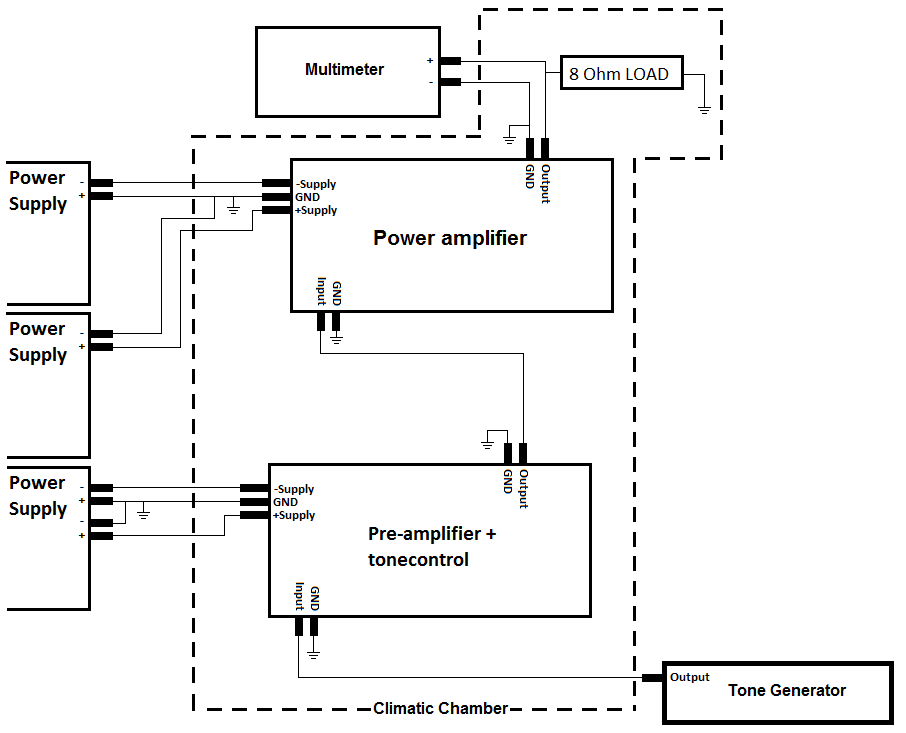
\includegraphics[scale=.8]{figures/filename}
	\flushleft 
	\caption{CAPTION\fxnote{Remember source}}
	\label{LABEL}
	\flushleft
	\textit{SOURCE}
\end{figure}

%--------- NOTES ------------------------------------------------------
%Fxnotes wont compile properly inside the figure, only in the caption.
%Filetype can be specified but isn't needed.

\noindent
\figref{LABEL}\\

\noindent
\Figref{LABEL}

\vspace{.5cm}
%Do not use \vspace{length} or \hspace{length} unless exceedingly necessary.

%--------- BIBLIOGRAPHY REF EKSAMPLE -----------------------------------
This reference only represents this line since it is before the punctuation mark\cite{YDing}. This next reference however represents the entire section. That is all of the preceding sentences in the entire section. This is due to the fact that it is now after the punctuation mark in the end of the section (this is not used in the middle of a section!).\cite{YDing}
%>>>>>>>>>>>>>>>PLEASE ALSO READ THE NOTE IN myBib.bib<<<<<<<<<<<<<<<<<<
\pagebreak	%||||||||
%	\section{Table Sample}

\begin{table}[H]
\caption{This Is a Table\label{LABEL}}
\begin{tabular}{|l|p{5cm}|l|l|l|}
  \hline
  \textbf{No.}&\textbf{Description}&\textbf{Min}&\textbf{Max}&\textbf{Requirements}\\
  \hline
  1 & Some Text & Some Text & Some Text & Some Text\\
    &           &           &           & Some More Text\\
    &           &           &           & Text Text\\
    &           &           &           & Text Text Text\\
  \hline
  2 & Some Text & Some Text & Some Text & Some Text\\
  \hline
  3 & 	By specifying the width of a column (|p\{5cm\}|) the cells
  		in that column will will not exceed	the specified width    %Enter is used only for clarity and will not affect the compiled output.
  		but instead expand downward.
  		
  		        & Some Text & Some Text & Some Text\\
  \hline
  4 & Some Text & Some Text & Some Text & Some Text\\
  \hline
  \multicolumn{2}{|l|}{Some Text} 	&	\multicolumn{3}{l|}{Some Text}\\
  \hline
  \multicolumn{2}{|l|}{Text Text} 	&	\multicolumn{3}{l|}{Text = Text}\\
  \multicolumn{2}{|l|}{}			&	\multicolumn{3}{l|}{Text = Text}\\
  \multicolumn{2}{|l|}{}			&	\multicolumn{3}{l|}{Text = Text}\\
  \multicolumn{2}{|l|}{}			&	\multicolumn{3}{l|}{Text = Text}\\
  \multicolumn{2}{|l|}{}			&	\multicolumn{3}{l|}{Text = Text}\\
  \hline
  \multicolumn{2}{|l|}{Some Text} 	&	\multicolumn{3}{l|}{Teeeexxtt}\\
  \multicolumn{2}{|l|}{}			&	\multicolumn{3}{l|}{\LaTeX}\\
  \hline      
\end{tabular}
\end{table}

\noindent
\tabref{LABEL}\\

\noindent
\Tabref{LABEL}

\pagebreak	%||||||||
%	\section{Equation Sample}

Ohms Law:
\begin{flalign}
  U &= I \times R \unit{\volt}
  \label{eq1}
\end{flalign}
%
Some explanation:
\begin{flalign}
  [Equation] &= [Number] \unit{Unit}
  \label{eq2}
\end{flalign}
%
Some explanation:
\begin{flalign}
  [Equation] &= [Number] \unit{Unit}
  \label{eq3}
\end{flalign}
%
Some explanation:
\begin{flalign}
  [Equation] &= [Number] \unit{Unit}
  \label{eq4}
\end{flalign}
%
Some explanation:
\begin{flalign}
  [Short Equation] &= [Number] \unit{Unit}
  \label{eq5}\\ %<-------------------------------------------------| Remember linebreak AFTER
  [Somewhat Longer Equation] &= [Number] \unit{Unit} %             | label when writing multiple
  \label{eq6}\\ %<-------------------------------------------------| equations.
  [Somewhat Quite a Lot Longer Equation] &= [Number] \unit{Unit}
  \label{eq7}
\end{flalign}
%
%
\eqref{eq1}\\
%
\eqrefTwo{eq1}{eq2}\\
%
\eqrefThree{eq1}{eq2}{eq3}\\
%
\eqrefFour{eq1}{eq2}{eq3}{eq4}\\
%
\eqrefFive{eq1}{eq2}{eq3}{eq4}{eq5}\\
%
\eqrefSix{eq1}{eq2}{eq3}{eq4}{eq5}{eq6}\\
%
\eqrefSeven{eq1}{eq2}{eq3}{eq4}{eq5}{eq6}{eq7}\\
%
\Eqref{eq1}\\
%
\EqrefTwo{eq1}{eq2}\\
%
\EqrefThree{eq1}{eq2}{eq3}\\
%
\EqrefFour{eq1}{eq2}{eq3}{eq4}\\
%
\EqrefFive{eq1}{eq2}{eq3}{eq4}{eq5}\\
%
\EqrefSix{eq1}{eq2}{eq3}{eq4}{eq5}{eq6}\\
%
\EqrefSeven{eq1}{eq2}{eq3}{eq4}{eq5}{eq6}{eq7}
%
\pagebreak	%||||||||
%|||||||												 ||||||||
%||||||||||||||||||||||||||||||||||||||||||||||||||||||||||||||||
%||||||||||||||||||||||||||||||||||||||||||||||||||||||||||||||||


%implementing front page:
\clearpage
\thispagestyle{empty}

\begin{figure}[H]
	\raggedleft
		
\includegraphics[width=0.2\textwidth]{figures/aaulogo-da.png}
\end{figure} 
\vspace*{\fill} 
\begin{center}	
\begin{Huge}
\textbf{Prædiktiv model til kapacitetsudnyttelse}\\
\vspace{5 mm}
P$5$ Semestersprojekt - Efteråret $2016$\\
\vspace{3 mm}
\end{Huge}
{\Large Gruppe $5405$}
\end{center}
\vspace*{\fill}

\begin{center}
\line(1,0){400}
\end{center}


%clears one or two pages to make the document start on right hand side:
%\cleardoublepage

%numbers the pages with Roman numeral - starts from "i":
\frontmatter

%implementing title sheet:
%\begin{document} 
\thispagestyle{empty}
%\begin{titlepage}
\begin{nopagebreak}
	{\samepage 
		
		\begin{tabular}{r}
			\parbox{\textwidth}{  \raisebox{11mm}{
\includegraphics[height=2cm]{figures/aaulogo-da.png}}
				\hfill \hspace{2cm} \parbox{8cm}{\begin{tabular}{l} %4.90
						{\small \textbf{\textcolor{MidnightBlue}{{$5$. Semester}}}}\\
						{\small \textbf{\textcolor{MidnightBlue}{School of Medicine and Health}}}\\
						%{\small \textbf{\textcolor{MidnightBlue}{}}}\\ 
						{\small \textbf{\textcolor{MidnightBlue}{Sundhedsteknologi}}}\\
						{\small \textcolor{NavyBlue}{Fredrik Bajers Vej $7$A}} \\
						{\small \textcolor{NavyBlue}{$9220$ Aalborg}} \\
						%{\small \textcolor{NavyBlue}{\emph{http://www.smh.aau.dk/}}}
			\end{tabular}}}
		\end{tabular}
		
		\begin{tabular}{cc}
			\parbox{7cm}{
				\begin{description}

%\item {Titel:}
%
%Prædiktiv model til kapacitetsudnyttelse\\

\item {Tema:} 

\small{
Klinisk teknologi
}

\end{description}

\parbox{8cm}{

\begin{description}
\item {Projektperiode:}\\
   P$5$, Efteråret $2016$\\
   
\item {Projektgruppe:}\\
  $5405$\\
  
\item {Medvirkende:}\\
Linette Helena Poulsen\\
Maria Kaalund Kroustrup\\
Nirusha Jeevanadan \\
Rolf Oberlin Hansen\\
Sageevan Sayananthan \\
Sebastian Munk \\

\hspace{2cm}
\item {Vejleder:}\\
Hovedevejleder: Pia B. Elberg \\
Kliniske vejleder: Sten Rasmussen \\
Klinisk bivejleder: Christian Kruse. \\  
\end{description}

}
\begin{description}
\item {Sider: XX}
\item {Appendikser: XX}
\item {Afsluttet:}
\end{description}
\vfill } &
\parbox{7cm}{
  \vspace{.15cm}
  \hfill 
  \begin{tabular}{l}
  {Synopsis:}\bigskip \\
  \fbox{
    \parbox{6.5cm}{\bigskip
     {\vfill{\small Overlæge Sten Rasmussen udtaler, at omfanget af kapacitetsmangel på ortopædkirurgisk afdeling på Aalborg Universitetshospital opleves stigende og tiltagende. Hertil forekommer der i år $2017$ en ny budgetaftale, der omhandler hurtigere udredning. Dette forventes at kunne skabe udfordringer for patientplanlægningen og kapacitetsudnyttelsen. Ubalance i kapacitetsudnyttelsen kan medvirke til komplikationer ift. arbejdsvilkår og patientsikkerhed. Herved kan en effektivisering af planlægningen medvirke til at opretholde en balance i kapacitetsudnyttelsen. En mulig løsning til dette kan være anvendelse af prædiktiv modellering til estimering af elektive patienters indlæggelsesvarighed. Det kan konkluderes, at en prædiktiv model kan anvendes til at estimere indlæggelsesvarigheden. Det er på baggrund af denne projektrapport ikke muligt at vurdere præcisionen af denne model, hvorfor yderligere studier er påkrævet.
     \bigskip}}
     }}
   \end{tabular}}
\end{tabular}} \vspace{1.3cm}
\raggedleft
\textit{\tiny Offentliggørelse af rapportens indhold, med kildeangivelse, må kun ske efter aftale med forfatterne.}\nopagebreak
\\
\end{nopagebreak}
%\end{titlepage}
%\end{document}
 %	\cleardoublepage

% FORORD OG LÆSEVEJLEDNING
%\chapter*{Forord og læsevejledning}

\section*{Forord}
Dette projekt er udarbejdet af gruppe $16$gr$5405$, $5$. semesters studerende på ingeniøruddannelsen sundhedsteknologi på Aalborg Universitet. Projektet er udarbejdet i perioden $2$. september til $19$. december år $2016$. Projektforslaget er stillet af Sten Rasmussen, overlæge på ortopædkirurgisk afdeling på Aalborg Universitetshospital, og omhandler prædiktiv modellering til forudsigelse af indlæggelsesvarigheden for patienter mhp. at effektivisere planlægningen. 


Vi vil gerne takke hovedevejleder Pia B. Elberg, kliniske vejleder Sten Rasmussen samt kliniske bi-vejleder Christian Kruse for vejledning og feedback gennem hele projektperioden. Derudover vil vi give en særlig tak til ortopædkirurgisk afdeling på Aalborg Universitetshospital for samarbejdet. 


\section*{Læsevejledning}
Rapporten er inddelt i fem kapitler. Det første kapitel indeholder projektets indledning samt den initierende problemstilling, der ligger til grund for problemanalysen, som fremgår af andet kapitel. Metoden beskrives i tredje kapitel. Fjerde kapitel analyserer implementeringen af en prædiktiv model på ortopædkirurgisk afdeling ift. forudsigelse af indlæggelsesvarighed for patienter mhp. planlægning af disse. Det fjerde kapitel er syntese, der indeholder en diskussion, konklusion samt perspektivering af projektet. Kapitlerne efterfølges af bibliografi samt bilag. 


Til håndtering af kilder anvendes Vancouver-metoden. De anvendte kilder nummereres i kantede parenteser. Er referencen placeret efter et punktum i en sætning, tilhører den hele afsnittet. Er referencen placeret før et punktum, tilhører den sætningen. Er der placeret flere referencer efter hinanden, betyder dette, at der er anvendt flere referencer til den pågældende sætning eller afsnit. Referencer til bilag er ligeledes indsat i kantede parenteser og er placeret efter samme metode som kilder. 

Forkortelser er skrevet ud ved første anvendelse, hvorefter forkortelsen er skrevet i parentes. Denne forkortelse anvendes herefter fremadrettet i rapporten. 


Rapporten er udarbejdet i \LaTeX, herudover anvendes MATLAB $2016$b til databehandling samt visualisering af grafer. 
 \cleardoublepage

%the '*' allows the tableofcontents be excepted from the actual table of contents.
\tableofcontents*
%\cleardoublepage

%numbers the pages with Arabic numeral - starts from 1.
\mainmatter

%---------------------------INPUTS-------------------------------


% INDLEDNING

\chapter{Indledning}


Flere danske hospitalsafdelinger oplever i perioder at have flere patienter end der er kapacitet til, i form af mangel på sengepladser, personale eller rum\cite{Company2013}. Overskridelsen af kapaciteten resulterer bl.a. i, at personalet får mindre tid pr. indlagt patient, hvilket kan medføre gener for både personalet og patienter.\cite{Kjeldsen2015} I budgetfordelingen for Aalborg Universitetshospital i år 2017 indgår det, at ventetiden på en operation for elektive patienter skal reduceres fra 57 dage til 50 dage\cite{Budget2016}. Dette forventes at medføre, at det daglige antal elektive patienter, der indlægges, vil skabe en reducering i antallet af ledige sengepladser til akutte patienter. 

Et estimat fra 2016 indikerer, at procentdelen af danskere over 65 år vil stige fra $29~\%$ til $34~\%$ og dermed også antallet af patienter\cite{RegionNord2016}. En stigning i antallet af patienter vil i takt med kortere ventetid på behandling skabe et aktuelt problem ift. planlægning af indlæggelser samt kapacitetudnyttelse på ortopædkirurgisk afdeling. Ifølge en undersøgelse fra Dansk Sygeplejeråd, mener hver anden regionalt ansat sygeplejerske på tværs af regionerne, at den travle arbejdsdag påvirker patientsikkerheden\cite{Kjeldsen2015}. Foruden personalets øgede risiko for at begå fejl ift. behandlingen af patienter, kan der ligeledes opstå en sundhedsrisiko ved kapacitetsmangel. Manglen på fysisk kapacitet kan give anledning til at overflytte patienter til uhensigtsmæssige områder som f.eks. hosptialsgange\cite{Madsen2014}. Dermed er der opstået et aktuelt problem som vedrører kapacitetsmangel, og konsekvenserne af dette problem bør undersøges nærmere. Ved at udnytte kapaciteten på afdelingen opnås der mere sundhed for pengene\cite{Company2013}. På baggrund af dette opstilles følgende initierende problem:

\textit{Hvordan påvirkes ortopædkirurgisk afdeling på Aalborg Universitetshospital af ændringerne vedrørende kapacitetsudnyttelse og hvor udbredte er belægningsrelaterede problemer på afdelingen?}





% Der er i dag overbelægning på flere afdelinger på de danske hospitaler, hvoraf nogle afdelingerne berøres i hele og flere måneder ad gangen. \cite{2015} Overbelægning resulterer i, at sundhedspersonalet får mindre tid pr. indlagt patient. Ifølge en undersøgelse fra Dansk Sygeplejeråd, mener hver anden regionalt ansat sygeplejerske på tværs af regionerne, at den travle arbejdsdag går ud over patienternes sikkerhed \cite{Kjeldsen2015}. Et studie påviser, at ved blot én ekstra indlagt patient pr. sygeplejerske øges mortalitetsraten med $7~\%$ indenfor en indlæggelse på 30 dage \fxnote{Har stadig lidt svært ved om man kan forstå sætningen på den rigtige måde.} \cite{Aiken2014}. 

% Foruden sundhedspersonalets øgede risiko for at begå fejl ift. behandlingen af patienter, er der ligeledes en sikkerhedsrisiko forbundet ved overbelægning på hospitalerne. De ekstra patienter, der ligger på stuerne, gangene og vaskerummene, pga. overbelægning, er en større udfordring ved evakuering under brand. Pladsmangel, som medfører, at patienterne opholder sig i vaskerummene og på gangene, bevirker desuden til, at patienterne oplever et skærpet privatliv. \cite{Madsen2014}

% Aalborg universitetshospital har i et tidligere projekt indsamlet data fra $1.000$ hospitalsindlæggelser. Disse data inkluderer blodprøveanalyser og knoglescanninger (DXA), hvilket formodes at kunne anvendes til udvikling af en prædiktiv model, der kan estimere indlæggelsesvarigheden blandt patienter. Denne rapport vil på baggrund af dette undersøge, hvorvidt det er muligt at forudsige indlæggelsesvarigheden ved brug af machine learning. \fxnote{mangler stadig noget om begrundelsen for valg af machine learning}



% \section{Initierende problemstilling} \fxnote{Dette er ikke den endelige problemstilling}
% Hvordan påvirkes personalet og patienterne af overbelægning på hospitaler, og hvilke konsekvenser har overbelægning i forhold til sikkerheden på afdelingerne?
% Hvilke typer af machine learning findes der, samt hvor benyttes det i dag?



% PROBLEMANALYSE
\chapter{Problemanalyse}
\section{Kapacitet} \label{kap}
% Skriv ift kapacitet (ift sengepladser, persona - hvilken betydning har hhv. 95 \% kapacitet mod 105 \%)
Kapacitetudnyttelse betegner forholdet mellem aktivitet og kapacitet. Aktivitet omhandler patient og kontakt, herunder består kontakt af forundersøgelse, behandling og kontrol. Kapacitet omfatter antallet af personale, udstyr og rum, hvor personalet består af læger, sygeplejersker og sekretærer. Udstyret beskriver antallet af maskiner på en afdeling og antallet af rum beskriver opbevarelsen af udstyret. Den samlede kapacitetsudnyttelse er defineret ud fra, at der produceres mest muligt for de investerede ressourcer.\cite{Company2013} 

\begin{figure}[H]
	\flushleft 
	\centering
	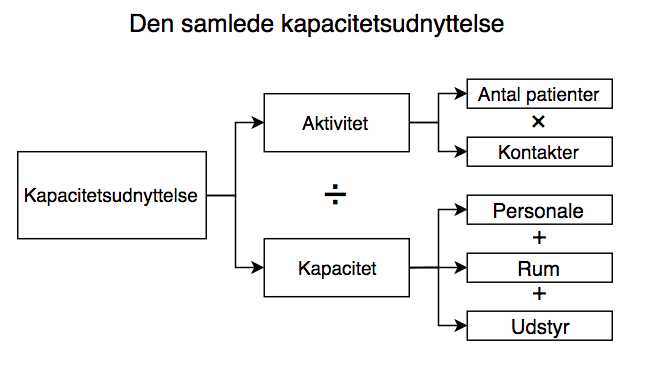
\includegraphics[scale=.65]{figures/Kapacitetsudnyttelse.png}
	\flushleft
	\caption{\textit{Den samlede kapacitetsudnyttelse som er definineret ved forholdet mellem aktivitet og kapacitet. Aktivitet omfatter antallet af patienter samt kontakter og kapacitet omfatter personale, rum og udstyr.}\cite{Company2013}}
	\label{kapacitet}
\end{figure}

\noindent
Ud fra \figref{kapacitet} fremgår det, at kapacitetsudnyttelse er forholdet mellem aktivitet og kapacitet. Dertil ses aktivitet som antal patienter multipliceret med kontakter. Kapaciteten udgør personale, rum og udstyr lagt sammen. Antallet af patienter, der repræsenterer en del af aktivitet beskriver ligeledes belægning på hospitalets afdelinger.\cite{Company2013} 

Belægning er defineret ud fra antallet af patienter, der er normeret til på en afdeling\cite{Heidmann2014}. Når en $100~\%$ belægning opnås, svarer dette til, at de disponible sengepladser på en afdeling er taget i brug. Ved en belægning på over $100~\%$ betyder det, at der er flere patienter end afdelingen er normeret til, hvilket vil sige, at afdelingen yder mere end der er kapacitet til. Ud fra \figref{kapacitet} vil dette betyde, at der ikke er ligevægt mellem aktivitet og kapacitet, hvilket i dette tilfælde vil forårsage kapacitetsmangel på afdelingen. Det kan derfor være nødvendigt, at personalet skal varetage flere patienter samt arbejdsopgaver, det kan ligeledes være nødvendigt at tilkalde ekstra personale for at opnå en balance i kapacitetsudnyttelsen.
Hvis der derimod er en belægning på under $100~\%$ er der omvendt færre patienter end afdelingen er normeret til. Dette betyder, at der er flere sengepladser end patienter, hvilket ligeledes fører til en ubalance i kapacitetsudnyttelsen. I denne situation er der mere personale end nødvendigt til at varetage de enkelte patienter, hvilket betyder, at der ikke er fuld udnyttelse af personalets arbejdskraft.\cite{Pauly1986} 

Det anses herved vigtigt, at der er balance mellem aktivitet og kapacitet, således de investerede ressourcer udnyttes optimalt. Det ønskes derfor at opnå en kapacitetsudnyttelse på $100~\%$. Ud fra dette vil der fremover undersøges betydningen af kapacitetsudnyttelse på ortopædkirurgisk afdeling på Aalborg Universitetshospital. 

\subsection{Ortopædkirurgisk afdeling}
Kapacitetsudnyttelse afhænger af det budget som hver afdeling har til rådighed. Dette budget udregner Sundhedsstyrrelsen ud fra diagnoserelaterede grupper (DRG). DRG anvendes til at analysere omkostninger og aktivitet på et hospital.\cite{DRG2016} Ortopædkirurgisk afdeling har et budget på $700.872.744$ kr, som svarer til 17,2 \% af det samlede budget for alle afdelinger på Aalborg Universitetshospital. Det samlede DRG for afdelingerne på Aalborg Universitetshospital er illusteret af \figref{DRG_budget}.\cite{Rasmussen2016}
Størstedelen af budgettet anvendes til personale- og patientudgifter, som svarer til hhv. 60 \% og 32 \%. Det resterende budget anvendes til bygninger, it, apparatur, inventar samt drift og service\cite{Noegletal2016}. 


\begin{figure}[H]
	\flushleft 
	\centering
	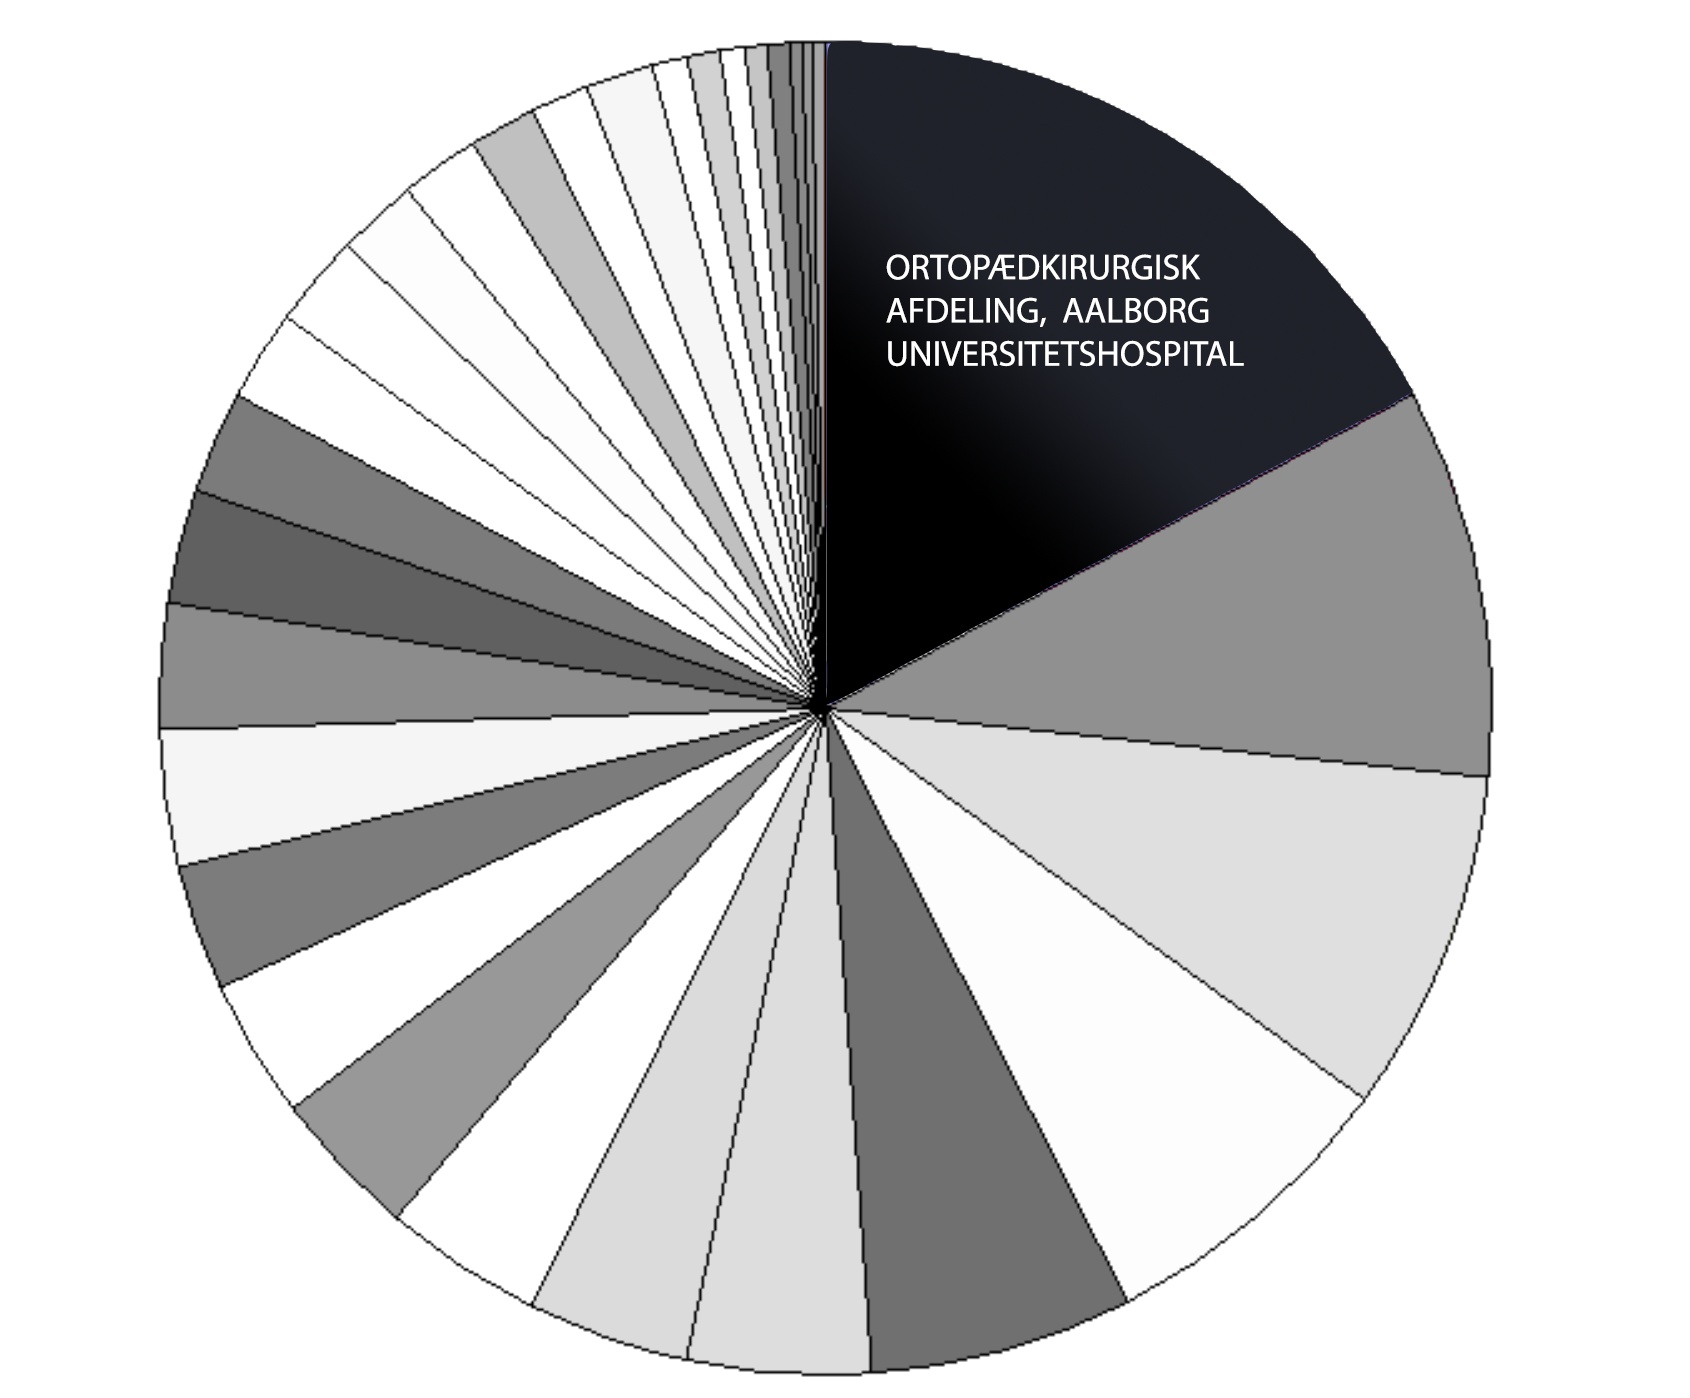
\includegraphics[scale=0.45]{figures/Ortopaeddiagram.png}
	\flushleft
	\caption{\textit{Fordeling af DRG for samtlige afdelinger på Aalborg Universitetshospital. Det fremgår, at ortopædkirurigisk afdeling har en større andel end de resterende afdelinger.}\cite{Rasmussen2016}}
	\label{DRG_budget}
\end{figure}


\subsubsection{Personalearbejde} 
% Hvordan opleves belægning generelt på OA på Aalborg UH? Hvordan varetages opgaver af personalet? Hvordan er vagtskifte? Hvor langt tid arbejdes der gennemsnitlig om dagen?
%Som beskrevet i \autoref{sec:kap} er personalet en del af kapacitet. Personalet ses som en væsentlig faktor for at udnytte kapaciteten effektivt. 
På ortopædkirurgisk afdeling på Aalborg Universitetshospital arbejder personalet i gennemsnit 37 timer om ugen\cite{Danske2015}. Vagterne kan variere fra XX til XX timer, hvoraf det både kan være nat- og dagvagter. Der er indlagt betalte pauser, hvilket betyder, at personalet skal være til rådighed under pausen. Pauserne er opdelt i XX om dagen. Afdelingen er delt op i XX vagthold og har vagtskifte hver XX time. Personalet varetager XX patienter om dagen. \fxnote{Vi mangler informationer for at kunne skrive dette færdigt.}

\subsubsection{Patientindlæggelse}
% Hvordan foregår indlæggelsen på OA på AUH? Hvornår indlæggelses patienterne (elektive patienter) og hvornår på dagen udskrives patienter (både elektive og akutte patienter) Hvor mange patienter hhv. akutte vs. elektive patienter? Hvad er deres buffer i forhold til elektive patienter, således der er plads til de akutte indlæggelser? indkaldes elektive patienter, hvis der er mindre akutte i en periode end der er estimeret til? Øges den normerede kapacitet under overbelægning ved at indkalde vikarbureau? (Altså tager man samme mængde elektive patienter ind.) 


Som beskrevet i afsnit \ref{kap} ønskes en $100~\%$ kapacitetsudnyttelse, dertil ønskes ligeledes en belægning på $100~\%$. 
For at opfylde dette skal der være ligevægt mellem antallet af sengepladser og patientindlæggelser. På ortopædkirurgisk afdeling har de XX sengepladser til rådighed, som er fordelt på XX afsnit.

Ortopædkirurgisk afdeling modtager både elektive samt akutte patienter. Elektive patienter omfatter både indlagte og ambulante patienter. Ved pludselig forværret tilstand kan elektive patienter skifte status fra elektiv til akut. Akutte patienter defineres som personer, der er henvist til hospitalet efter en akut opstået tilstand. Sammenlignes der med de resterende afdelinger på Aalborg Universitetshospital, har ortopædkirurgisk afdeling flest elektive indlæggelser.\cite{RegionNord2016} Elektive patienter indlægges i tidsrummet XX-XX og udskrives i tidsrummet XX-XX. Udskrivelsen af akutte patienter foregår i samme tidsrum. På afdelingen planlægges elektive patienter med forbehold for, at der er uforudsigelige indlæggelser af akutte patienter pr. XX. Herunder planlægges XX elektive patienter, således at der er plads til XX akutte patienter.\fxnote{Vi mangler informationer for at kunne skrive dette færdigt + tilføjelse af Sebastians grafer (elektive/akuttte) + (indlæggelse/udskrivelse)}
\section{Ubalance i kapacitetsudnyttelse}
Ved kapacitetsmangel på ortopædkirurgisk afdeling forekommer en omstrukturering af personalets arbejdsopgaver, som sikre patientens behov, opretholdelse af kvalitet og udnyttelse af kompetencer. Dette er med henblik på at opnå en balance mellem de ressourcer og de krav, der stilles i den pågældende situation.\cite{Bjerg2016}  %Generelt er personalet den begrænsende faktor for planlægning og kapacitetsudnyttelse\cite{Company2013}. 

\subsection{Arbejdsvilkår} \label{Per_sik}
%Hvordan påvirkes personalets arbejdsrutiner ved kapacitetsmangel? Hvor længes må deres arbejdsdag maksimalt være? Stiger antallet af fejl når personalet varetager en større arbejdsbyrde end planlagt? Hvor omkostningsfuldt er det? 

I tilfælde af kapacitetsmangel er der udarbejdet en arbejdstilrettelæggelse af Region Nordjylland for personalet på ortopædkirurgisk afdeling. Ved kapacitetsmangel påtager lederen, eller dennes stedfortræder, ansvaret for at finde en løsning på dette problem. Dette kan betyde, at det afgående vagthold skal blive indtil en midlertidig løsning er fundet eller en tidligere indkaldelse af det næste vagthold. I nogle tilfælde kan det være nødvendigt at låne ressourcer fra andre afsnit eller indkalde personale fra vikarbureauet. Derudover undersøges det, hvorvidt behandlingen af elektive patienter kan aflyses.\cite{Bjerg2016} 

Ved overarbejde må en arbejdsuge for en sygeplejerske, ifølge arbejdstidsaftalen indgået med Dansk Sygeplejeråd, ikke overstige 48 timer\cite{Danske2015}. \fxnote{Spørgsmål til sygeplejersker: Hvordan prioriteres pauser under overbelægning?} Hvis sundhedspersonalet er nødsaget til at arbejde længere end den normale arbejdstid, viser dette sig at have en negativ indvirkning på personalets arbejdesopgaver\cite{Dinges2004}. Overarbejde kan resultere i en presset arbejdsdag og dermed en forringet kvalitet af behandlingen\cite{Kjeldsen2015}. Dertil mener hver anden regionalt ansat sygeplejerske på tværs af regionerne, at den travle arbejdsdag påvirker patienternes sikkerhed\cite{Kjeldsen2015}.

%Den større patientbyrde, der skal varetages ved en belægning over 100\%, medvirker til en øget arbejdsbyrde for det tilstedeværende personale.\fxnote{Spørgsmål til sygeplejersker: Hvor mange patienter skal i under normale omstændigheder varetage? Og hvordan fungerer det under overbelægning? Fordeles de enkelte patienter mellem jer?} \cite{Dinges2004,Aiken2002,Madsen2014}
%Det er forsøgt at kapacitsoptimere, med en reduktion af sengepladser på $30~\%$ i perioden $1996$ til $2011$ \cite{Dinges2004,Aiken2002,Madsen2014} 


\subsection{Patientsikkerhed}
%Hvordan påvirker kapacitetsmangel ift. brandsikkerhed? Laver personalet flere fejl, som går ud over patienterne ved overbelægning? Hvordan fungerer omrokering af patienter (gangarealer, vaskerum ect.)? Hvor omkostningsfuldt er det for OA’s budget? brandsikkerhed og Genindlæggelse
Under perioder med kapacitetsmangel er det ofte nødvendigt at overflytte patienter til andre afdelinger, gangarealer eller fyldte stuer, herved er det ofte patienter, der snart udskrives, der overflyttes. \fxnote{Sygeplejersker: Vi vil gerne høre om der prioriteres i forhold til hvilke patienter der flyttes. Er der en bestemt afdeling i flytter patienterne over på eventuelt en afdeling der ligner ortopædkirurgisk?} Overflytningen kan belaste både fysiske og psykiske forhold for patienter såvel som pårørende\cite{Heidmann2014}. Herunder kan skærpet privatliv forekomme hos patienter, der er flyttet til gangarealer eller fyldte stuer\cite{Madsen2014}. 

Som nævnt i afsnit \ref{Per_sik} forringes kvaliteten af behandlingen ved overarbejde, dertil ses det ligeledes, at mortalitetsraten øges med $1,2~\%$ ved en overskridelse af belægningen med $10~\%$, ifølge et dansk studie fra år $2014$\cite{Madsen2014}. Hertil understreges det, at der kan være ukendte parametre, der påvirker mortalitetsraten, og det nødvendigvis ikke er belægning, der er den primære årsag til en øget mortalitet. For at undgå forringet kvalitet af behandling forsøges det at få patienterne udskrevet tidligere, således et ønske om balance mellem aktivitet og kapacitet opnås.

%\fxnote{Tidligere afsnit: Hvordan er fordelingen af elektive og akutte patinter? Kan elektive patienter tages ind før der er normalbelægning?} 

Der tilkaldes en brandvagt til afdelingen, hvis en belægning over $100~\%$ har fundet sted i over $4$ timer for således at sikre patienterne ved evakuering under brand. En brandvagt kan højest overvåge to afdelinger på samme etage, hvorfor det kan være nødvendigt, at der indkaldes flere. Det er afdelingens ansvar at afvikle belægningsproblemet og kapacitetsmanglen hurtigst muligt ved at udskrive patienter eller overflytte patienter til andre afdelinger. \fxnote{Har skal indsættes hvis de har et samarbejde med en anden afdeling} Hver gang der tilkaldes en brandvagt faktureres dette af Aalborg Universitetshospital.\cite{Beredskab2016}



\section{Omfang af belægning}
På ortopædkirurgisk afdeling på Aalborg Universitetshospital ses en varierende belægningsgrad fra måned til måned. Belægningsgraden er antallet af disponible senge i brug. På \figref{maxminbelaeg} ses den varierende belægning fra år $2014$ til $2015$ på ortopædkirurgisk afdeling. \cite{SDS2015}


\begin{figure}[H]
	\flushleft 
	\centering
	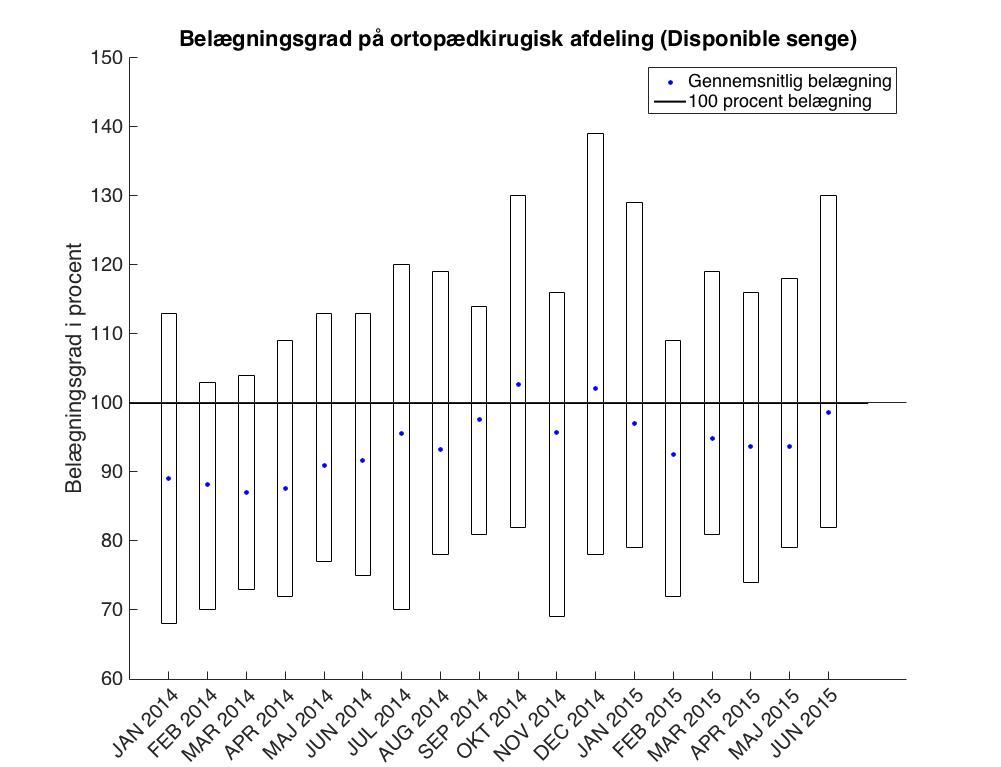
\includegraphics[scale=.45]{figures/maxminoverbelaeg.png}
	\label{maxminbelaeg}
	\flushleft
	\caption{\textit{Figuren illustrerer belægningsgraden over 18 måneder fra år $2014$ til $2015$ på ortopædkirurgisk afdeling på Aalborg Universitetshospital. Søjlerne viser belægning ift. $100\%$ belægning, dertil ses den gennemsnitlige belægning for hver måned som et punkt. \cite{SDS2015}}}
\end{figure}


Det fremgår af \figref{maxminbelaeg}, at ortopædkirurgisk afdeling oplever en belægning hhv. over og under én ønskede belægning på $100 \%$. I december måned år $2014$ ses en maksimal belægning på $1XX \%$ og en minimums belægning på $xx \%$. Dette indikerer, at ortopædkirurgisk afdeling oplever belægning over $100 \%$ i kortvarige perioder. Da \figref{maxminbelaeg} ikke viser belægningsperioden er det uvist om, hvorvidt belægningen over $100 \%$ opleves i timer eller flere dage. Der skal herudover tages forbehold for, at \figref{maxminbelaeg} både indeholder elektive samt akutte indlagte patienter, og derfor er uvist om, hvorvidt det er akutte patienter, der resulterer i en belægningsgrad på over $100 \%$. Der ses ligeledes en gennemsnitlig belægning pr. måned på \figref{maxminbelaeg}. Denne ses hyppigst under $100 \%$ belægning, hvortil der kun ses oktober samt december i år $2014$ med en gennemsnitlig belægning på over $100 \%$ belægning. Derved opleves der ikke en gennemsnitlig belægning på over $100 \%$ i $16$ ud af de $18$ oplyste måneder. \cite{SDS2015}


For at underbygge belægningsgraden yderligere, illustrerer \figref{antaldage} antal dage pr. måned med en belægningsgrad på over $100 \%$. Denne graf er udarbejdet ud fra ortopædkirurgisk afdeling over de samme 18 måneder fra år $2014$ til $2015$ som \figref{maxminbelaeg}. \cite{SDS2015} 

\begin{figure}[H]
	\flushleft 
	\centering
	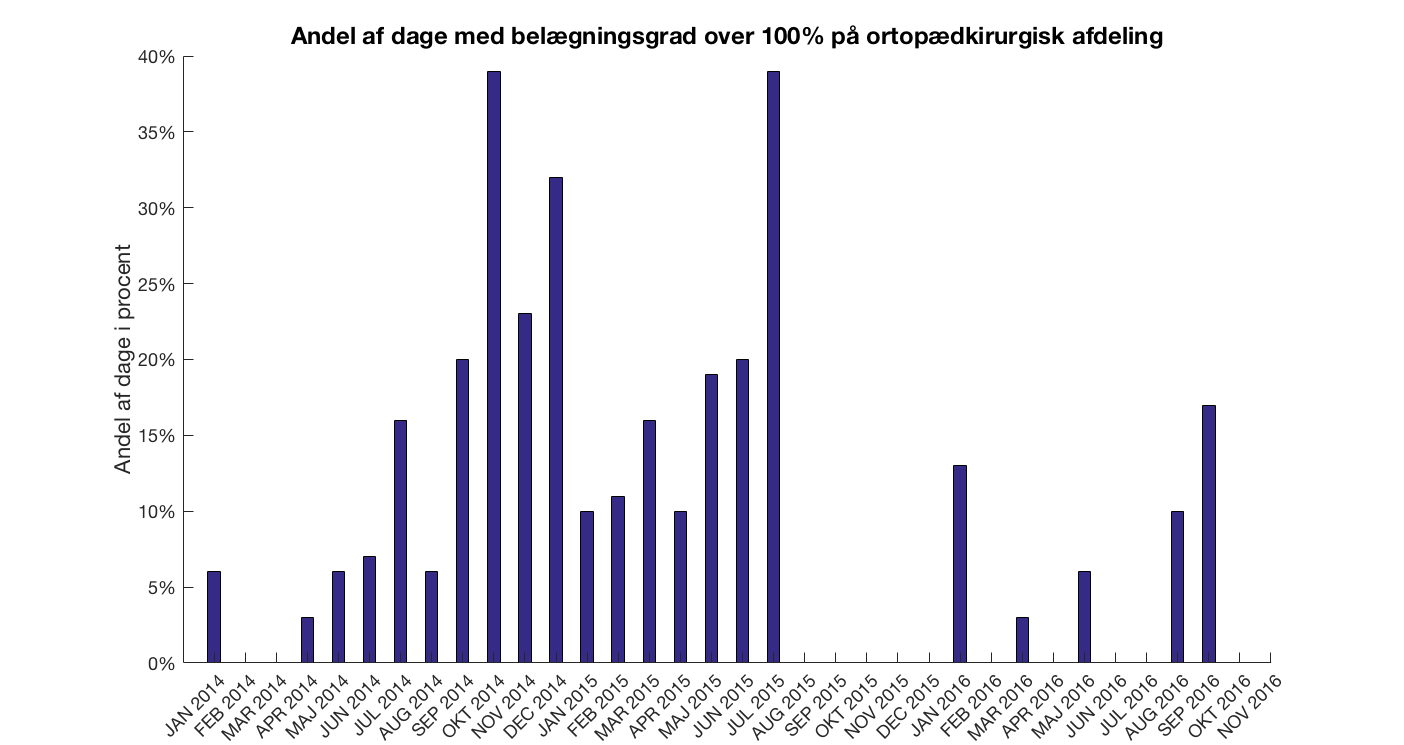
\includegraphics[scale=.7]{figures/antaldage.png}
	\label{antaldage}
	\flushleft
	\caption{\textit{Figuren illustrerer antal dage med en belægningsgrad over $100 \%$ fra januar 			$2014$ til juni $2015$ på ortopædkirugisk afdeling på Aalborg Universitetshospital. 					\cite{SDS2015}}}
\end{figure}


Af \figref{antaldage} ses det, at der i oktober måned år 2014 opleves en belægning på over $100 \%$ i 19 dage. Det vides dog ikke, hvorvidt der er tale om én ekstra eller flere patienter, der udgør en belægningsgrad på over $100 \%$, samt hvor længe patienterne er indlagt på afdelingen. Det ses i \figref{maxminbelaeg}, at der i oktober måned år 2014 opleves en belægning på $130 \%$, hvilket kan opholdes mod de 19 dage. Det skal understreges, at begge grafer er angivet i måneder, og det er derfor uvist om, hvor mange patienter, der er indlagt pr. dag. Derudover er figurerne, \figref{maxminbelaeg} og \figref{antaldage}, udarbejdet over 18 måneder, hvilket angiveligt ikke er en repræsentativ periode for at konkludere et reelt problem på afdelingen. Dertil vides det ikke om belægningsgraden over $100 \%$ opleves som værende et problem på ortopædkirurgisk afdeling på Aalborg Universitetshospital eller om det blot er et strukturerings problem. 
\section{Problemformulering}
\textit{Hvordan kan indlæggelsesvarigheden for patienter på ortopædkirurgisk afdeling på Aalborg Universitetshospital forudsiges med henblik på at opretholde en kapacitetsudnyttelse på 100 \%?}
%\subsection{Personale og patient}

\subsubsection{Konsekvenser af overbelægning}

Overbelægning på sygehuse samt forlængede arbejdsdage viser at have en negativ indvirkning på sundhedspersonale. Dette medfører en forhøget risiko for at lave fejl fra sundhedspersonalets side. Fejlene opstår hovedsagligt når personalet har arbejdsdage på mere end 12 timer. Ifølge i et dansk studie fra 2014, forøges risikoen for dødeligheden på hospitalet med ca. 1,2 \% ved en forøgelse i belægning på ti \%.







sygeplejersker er nødsaget til at have flere patienter pr. time (hvilket er nederen for begge parter)

Forringet kvalitet i forhold til operationer og medicinering 

Nedsat komfort for patienter (dårligt miljø)→ længere indlæggelsesperiode?

%\section{nyt afsnit om overbelægning - udkast}

I dette afsnit undersøges belægningsgraden på ortopædkirugisk afdeling på Aalborg Universitetshospital. Belægningsgraden er antallet af disponible senge i brug. På \figref{maxminbelaeg} ses belægningsgraden på ortopædkirugisk afdeling fra januar $2014$ til juni $2015$.\cite{SDS2015}

\begin{figure}[H]
	\flushleft 
	\caption{Belægningsgrad i procent på ortopædkirugisk afdeling}
	\centering
	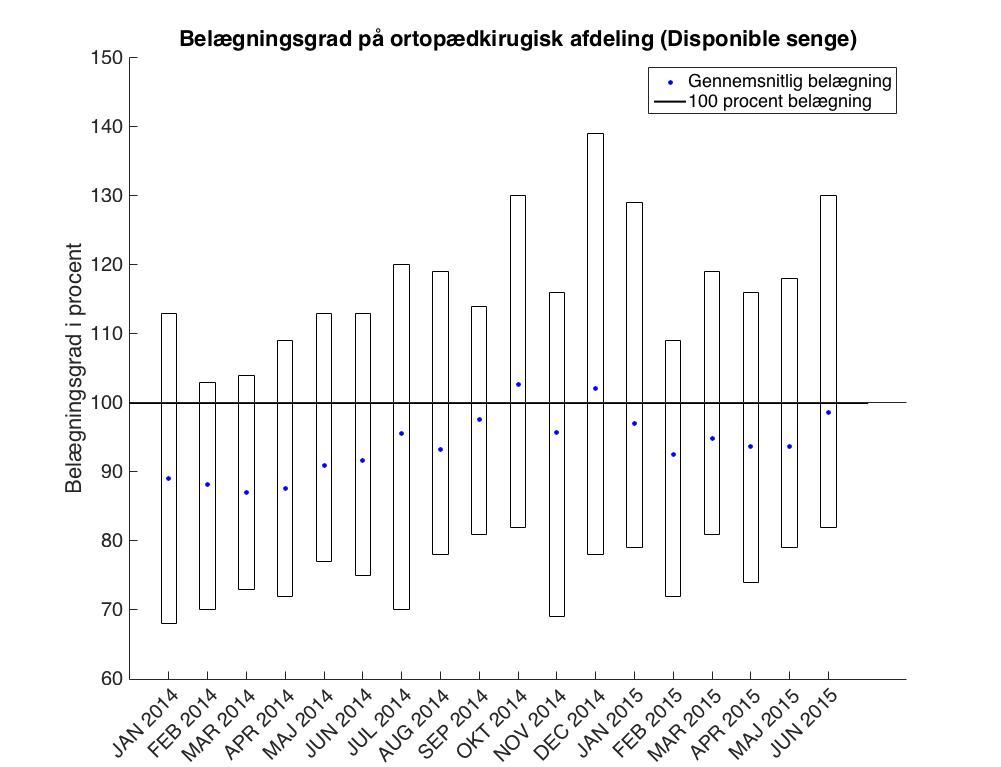
\includegraphics[scale=.45]{figures/maxminoverbelaeg.png}
	\label{maxminbelaeg}
	\flushleft
	\textit{Figuren viser minimums- og maksimumsbelægning på ortopædkirugisk, samt den gennemsnitlige belægning, fra januar $2014$ til juni $2015$ på ortopædkirugisk afdeling på Aalborg Universitetshospital.\cite{SDS2015}}
\end{figure}

Som det ses på \figref{maxminbelaeg} er den gennemsnitlige belægning på ortopædkirugisk afdeling typisk under $100$\%. Kun $2$ ud af $18$ måneder har en gennemsnitlig belægning over $100$\%. Det ses ligeledes at den maksimale belægning er over $100$\% i alle $18$ måneder. Dette tyder på at overbelægning på afdelingen forekommer i kortvarige episoder, frem for længerevarende perioder.\cite{SDS2015}

Dette underbygges af hyppigheden for overbelægning. \Figref{antaldage} viser antallet af dage, hvor ortopædkirugisk afdeling på Aalborg Universitetshospital har haft en belægningsgrad over $100$\%.\cite{SDS2015}

\begin{figure}[H]
	\flushleft 
	\caption{Antal dage med belægningsgrad over $100$\% på ortopædkirugisk afdeling}
	\centering
	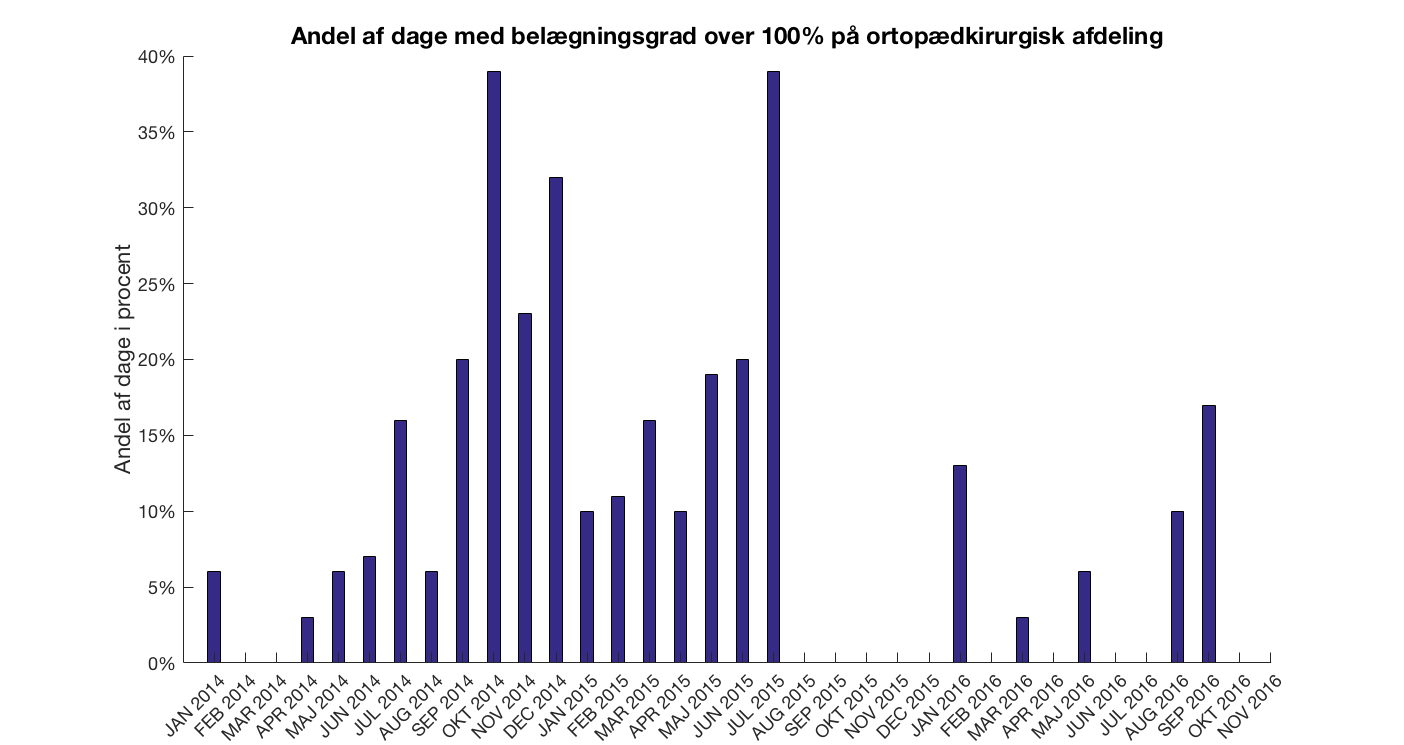
\includegraphics[scale=.7]{figures/antaldage.png}
	\label{antaldage}
	\flushleft
	\textit{Figuren antal dage med belægningsgrad over $100$\%, fra januar 2014 til juni 2015 på ortopædkirugisk afdeling på Aalborg Universitetshospital.\cite{SDS2015}}
\end{figure}
%%%%%% Mangler fxnote

%%% OMFLYTNING AF PATIENTER
%% Nogle af fxnotes skal skrives efter samtale med flere sygeplejersker
%% Der skal skrives noget om elektive patienter ud fra et tidligere et afsnit som ikke er skrevet endnu.

%%% TILRETTELÆGGELSE AF PERSONALE
%% Sygeplejersker: Hvor mange patienter skal i under normale omstændigheder varetage? Og hvordan fungerer det under overbelægning fordeles de enkelte patienter mellem jer? Erfaring?


%%% JURIDISKE PROBLEMSTILLINER:
%Hvis overbelægning er mere end 50 dage brydes loven (hvis det med elektive patienter kommer ind i omflytning af patienter.)
% Sygeplejerske/Sten/Økonomiafdeling: dette skal undersøges om det er fra det samlede budget eller om det bliver taget fra ortopædkirurgisk afdeling?
% Sygeplejersker: Hvordan prioriteres pauser under overbelægning

%%% OPSUMERING:
%%MANGLER KILDER PÅ NOGLE AF SÆTNINGERNE - kilderne skal tages når vi har fået svar fra sygeplejerskerne. 


\section{Konsekvenser og omkostninger ved overbelægning}
Ved overbelægning er det vigtigt, at situationen afvikles straks, da det bl.a. kan skabe problemer ift. arbejdsopgaver samt give et skærpet privatliv for patienten og forøgelse i mortaliteten. \cite{Madsen2014}
Ved overbelægning tilkaldes og tilrettelægges arbejdet for personalet, og der stræbes på at finde en balance mellem de eksisterende ressourcer, og de krav der stilles til den enkelte afdeling. \cite{Bjerg2016} Derudover omflyttes patienter ud fra nogle konkrete retningslinjer. \cite{Beredskab2016} Ved overbelægning skal der yderligere overholdes lovgivninger om sikkerhed og overenskomster for sundhedspersonalet. \cite{Beredskab2016}


\subsection{Tilrettelæggelse af personale} \label{Tilret}
Under overbelægning gælder en arbejdstilrettelæggelse som er udarbejdet af Region Nordjylland og omfatter ortopædkirurgisk afdeling. Dennes formål er, at sikre patientens behov, kvalitetssikring, udnyttelse af kompetencer med henblik på at finde en balance mellem ressourcerne og krav i den pågældende situation. Ved overbelægning påtager lederen eller dennes stedfortræder ansvaret for at finde en løsning. Dette betyder at det afgående vagthold skal blive indtil en midlertidig løsning er fundet. Derudover undersøges det om elektive patienter kan aflyses, og hvorvidt der bør indkaldes personale til at dække det manglede fremmøde. Dertil kan det være nødvendigt at indkalde det næste vagthold tidligere. Det kan blive en nødvendighed, at låne ressourcer fra andre afsnit eller indkalde personale fra vikarbureauet. Den sidste løsning er, at forlænge arbejdstiden for flere på det afgående vagthold til situationen kan varetages af de resterende. \cite{Bjerg2016}

\noindent 
Ved normale omstændigheder varetages XX antal patienter pr. sygeplejerske. De ekstra patienter, der behandles under overbelægning bliver fordelt mellem det tilstedeværende sundhedspersonale, og overskrider dermed den forventede patientbyrde. \fxnote{Sygeplejersker: Hvor mange patienter skal i under normale omstændigheder varetage? Og hvordan fungerer det under overbelægning fordeles de enkelte patienter mellem jer? Erfaring?}
Dette resulterer i, at sundhedspersonalet har kortere tid til den enkelte patient, hvorfor risikoen for fejl øges, hvilket betyder, at det ikke er muligt at give patienterne den nødvendige behandling efter det kirurgiske indgreb. \cite{Dinges2004} \cite{Aiken2002} Udover overbelægning har reduceringen af sengepladser på $30~\%$ medvirket til, at øge sygeplejerskernes arbejdsbyrde med $40~\%$ fra år 2001 til 2015. \cite{Kjeldsen2015}


Hvis sundhedspersonalet er nødsaget til at arbejde længere end den normale arbejdstid, viser dette sig at have en negativ indvirkning på personalet.\cite{Kjeldsen2015} \cite{Dinges2004} Undersøgelser viser, at dette resulterer i en presset arbejdsdag og dermed en forringet kvalitet i behandlingen. \cite{Kjeldsen2015} Et amerikansk studie har på baggrund af undersøgelser fra år 2002 påvist, at fejlene hovedsageligt opstår, når personalet har arbejdsdage på mere end 12 timer.\cite{Dinges2004}. Undersøgelsen skal ses i perspektiv med de danske overenskomster for sundhedspersonalet. Det fremgår dog af Dansk Sygeplejeråd, at hver anden regionalt ansat sygeplejerske på tværs af regionerne mener, at den travle arbejdsdag påvirker patienternes sikkerhed \cite{Kjeldsen2015}. Overbelægning medfører derfor gene for både personale og patienter. 
 
\subsection{Omflytning af patienter}
For ortopædkirurgisk afdeling på Aalborg Universitetshospital er der opstillet retningslinjer af Nordjyllands Beredskabsstyrelse for, hvordan overbelægningen varetages. Til at starte med, forsøges det at udfylde alle stuerne på afdelingen. Hvis dette ikke er muligt, flyttes patienter til andre hospitalsafdelinger. Når der ikke er plads på de andre hospitalsafdelinger, placeres patienterne i samtalerum og flugtvejsgange som en midlertidig nødløsning. \cite{Beredskab2016} De patienter, der overflyttes er ofte patienter, som er på grænsen til at blive udskrevet \fxnote{Sygeplejersker: Vi vil gerne høre om der prioriteres i forhold til hvilke patienter der flyttes. Er der en bestemt afdeling i flytter patienterne over på eventuelt en afdeling der ligner ortopædkirurgisk?}.


\noindet
Overflytningen og ophold i samtalerum samt flugtvejsgange bevirker til, at patienterne oplever et skærpet privatliv. \cite{Madsen2014} Derudover kan det belaste fysiske og psykiske forhold for patienterne såvel som pårørende. \cite{Heidmann2014} Som nævnt i afsnit \ref{Tilret} øges risikoen for fejl ved overbelægning og dertil ses det at mortaliteten øges med $1,2~\%$ ved en overskridelse af sengebelægningskapaciteten på $10~\%$ ifølge et dansk studie fra år 2014. \cite{Madsen2014} Hertil understreges det, at der kan være flere parametre, der påvirker mortaliteten og det nødvendigvis ikke er overbelægning der er den primære årsag til øget mortalitet. Overbelægning giver derfor et forøget pres for at få patienterne udskrevet, således at der opnås en normalbelægning. \fxnote{Tidligere afsnit: Hvordan er fordelingen af elektive og akutte patinter? Kan elektive patienter tages ind før der er normalbelægning?}.


\subsection{Juridiske problemstillinger}
Udover omstrukturering af arbejdsopgaver samt omflytning af patienter, er der nogle juridiske problemstillinger, som skal overholdes for at disse ændringer er lovmæssigt sikre. Dette medvirker tilkaldelse af brandvagter for at skærpe sikkerheden ift. evakuering under brand. Derudover er det samtidigt vigtigt, at det bestræbes på, at overholdelse løn- og overenskomsterne for sundhedspersonalet.

\subsubsection{Brandsikkerhed}
Ved opdagelse af et belægningsproblem kontaktes en brandvagt, således at brandvagten kan være tilgængelig på afdelingen så snart overbelægningen finder sted. Hvis normal belægningstilstand er mulig inden for fire timer efter overbelægningen påbegyndes, er det ikke nødvendigt at tilkalde en brandvagt. En brandvagt kan højst overvåge to afdelinger på samme etage, hvorfor det kan være nødvendigt at der indkaldes flere. Det er afdelingens ansvar, at afvikle overbelægningen hurtigst muligt ved at udskrive patienter eller overflytte patienter til sengestuer på andre afdelinger. \cite{Beredskab2016} Foruden at være et juridisk problem, fratages der penge fra det overordnede budget for ortopædkirurgisk afdeling hver gang en brandvagt tilkaldes. \fxnote{Sygeplejerske/Sten/Økonomiafdeling: dette skal undersøges om det er fra det samlede budget eller om det bliver taget fra ortopædkirurgisk afdeling?} 

\subsubsection{Overenskomster}
Som tidligere nævnt i afsnit \ref{Tilret}, forlænges sundhedspersonalets arbejdsdag under overbelægning. En normal arbejdsuge for danske sygeplejersker er 37 timer. I tilfælde af overarbejde må en arbejdsuge for en sygeplejerske, ifølge arbejdstids aftalen indgået med Dansk Sygpelerråd, ikke overstige 48 timer. Planlægning af en sygeplejerskes normalarbejde skal derudover finde sted 24 timer før fremmøde, hvilket ikke inkluderende overarbejde. \cite{Danske2015} \fxnote{Sygeplejersker: Hvordan prioriteres pauser under overbelægning} Dette medfører nogle juridiske overvejelser, som skal tages i betragtning når sundhedspersonalet tilkaldes ekstraordinært således at overenskomster og brandsikkerhed overholdes. 


\subsubsection{Opsummering}
\fxnote{MANGLER KILDER PÅ NOGLE AF SÆTNINGERNE.}
Overbelægning medfører at sundhedspersonalets arbejdsbyrde forøges, hvilket resulterer i kortere tid til den enkelte patient, hvormed den tilsigtede pleje svækkes. \cite{Dinges2004} \cite{Aiken2002} Derudover sker der flere fejl når personalet er til rådighed længere end den planlagte arbejdstid.\cite{Dinges2004} Omflytningen af patienter skaber et skærpet privatliv og kan belaste patienten både fysisk og psykisk. \cite{Madsen2014} \cite{Heidmann2014} Dette kan skabe et øget pres for at få patienterne udskrevet for hurtigst muligt at opnå en normalbelægning. Udover disse konsekvenser skal de lovmæssige regler overholdes, hvilket kan være omkostningsfuldt for ortopædkirurgisk afdelingen, ift. indkaldelse af brandvagter samt overenskomster for sundhedspersonalet. \cite{Beredskab2016}\cite{Danske2015} Overbelægning er derfor omkostningsfuldt og et problem for ortopædkirurgisk afdeling.

%\section{Omfang af belægning}
På ortopædkirurgisk afdeling på Aalborg Universitetshospital ses en varierende belægningsgrad fra måned til måned. Belægningsgraden er antallet af disponible senge i brug. På \figref{maxminbelaeg} ses den varierende belægning fra år $2014$ til $2015$ på ortopædkirurgisk afdeling. \cite{SDS2015}


\begin{figure}[H]
	\flushleft 
	\centering
	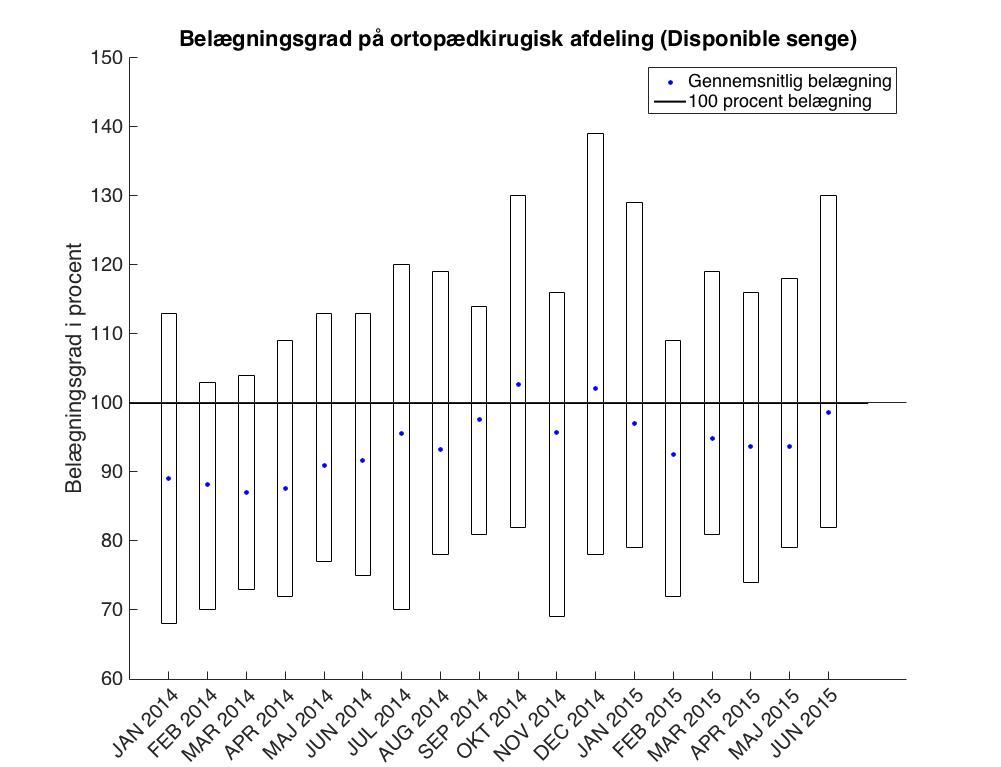
\includegraphics[scale=.45]{figures/maxminoverbelaeg.png}
	\label{maxminbelaeg}
	\flushleft
	\caption{\textit{Figuren illustrerer belægningsgraden over 18 måneder fra år $2014$ til $2015$ på ortopædkirurgisk afdeling på Aalborg Universitetshospital. Søjlerne viser belægning ift. $100\%$ belægning, dertil ses den gennemsnitlige belægning for hver måned som et punkt. \cite{SDS2015}}}
\end{figure}


Det fremgår af \figref{maxminbelaeg}, at ortopædkirurgisk afdeling oplever en belægning hhv. over og under én ønskede belægning på $100 \%$. I december måned år $2014$ ses en maksimal belægning på $1XX \%$ og en minimums belægning på $xx \%$. Dette indikerer, at ortopædkirurgisk afdeling oplever belægning over $100 \%$ i kortvarige perioder. Da \figref{maxminbelaeg} ikke viser belægningsperioden er det uvist om, hvorvidt belægningen over $100 \%$ opleves i timer eller flere dage. Der skal herudover tages forbehold for, at \figref{maxminbelaeg} både indeholder elektive samt akutte indlagte patienter, og derfor er uvist om, hvorvidt det er akutte patienter, der resulterer i en belægningsgrad på over $100 \%$. Der ses ligeledes en gennemsnitlig belægning pr. måned på \figref{maxminbelaeg}. Denne ses hyppigst under $100 \%$ belægning, hvortil der kun ses oktober samt december i år $2014$ med en gennemsnitlig belægning på over $100 \%$ belægning. Derved opleves der ikke en gennemsnitlig belægning på over $100 \%$ i $16$ ud af de $18$ oplyste måneder. \cite{SDS2015}


For at underbygge belægningsgraden yderligere, illustrerer \figref{antaldage} antal dage pr. måned med en belægningsgrad på over $100 \%$. Denne graf er udarbejdet ud fra ortopædkirurgisk afdeling over de samme 18 måneder fra år $2014$ til $2015$ som \figref{maxminbelaeg}. \cite{SDS2015} 

\begin{figure}[H]
	\flushleft 
	\centering
	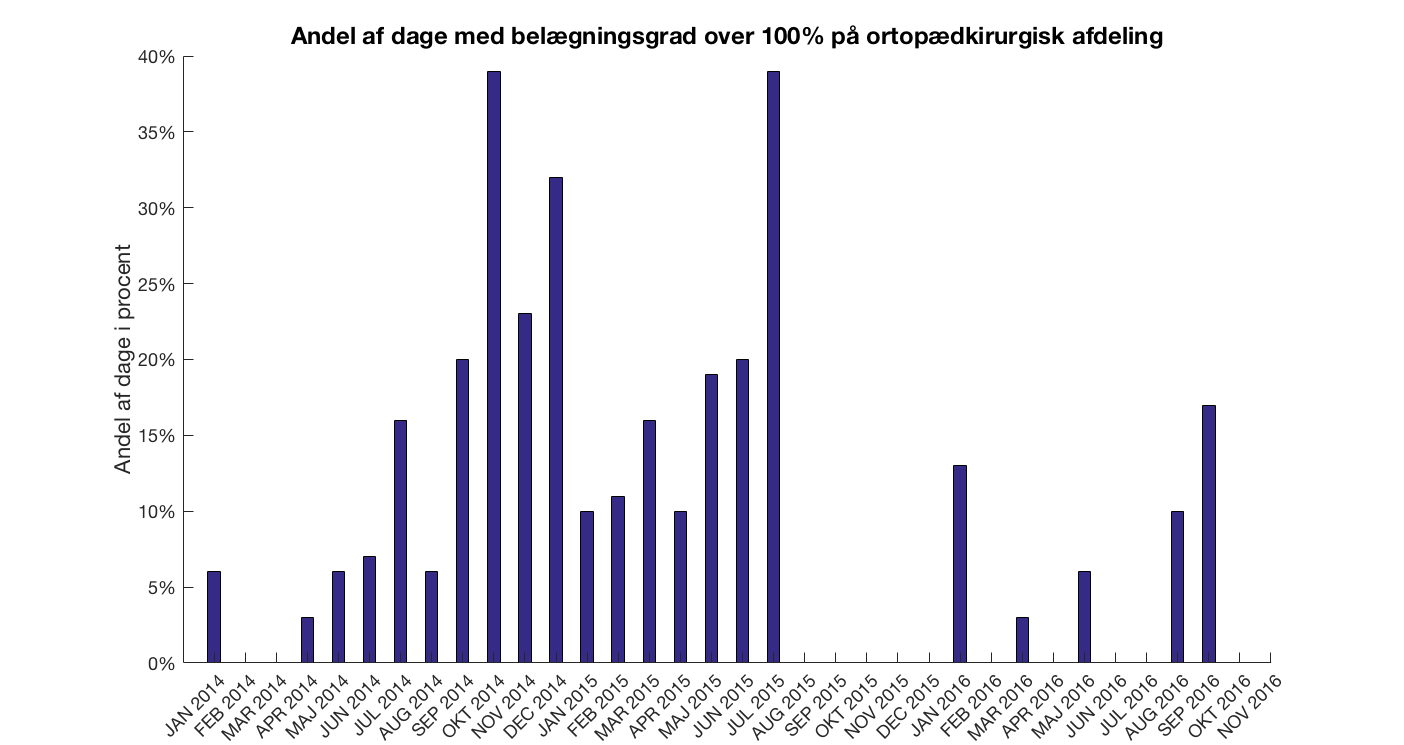
\includegraphics[scale=.7]{figures/antaldage.png}
	\label{antaldage}
	\flushleft
	\caption{\textit{Figuren illustrerer antal dage med en belægningsgrad over $100 \%$ fra januar 			$2014$ til juni $2015$ på ortopædkirugisk afdeling på Aalborg Universitetshospital. 					\cite{SDS2015}}}
\end{figure}


Af \figref{antaldage} ses det, at der i oktober måned år 2014 opleves en belægning på over $100 \%$ i 19 dage. Det vides dog ikke, hvorvidt der er tale om én ekstra eller flere patienter, der udgør en belægningsgrad på over $100 \%$, samt hvor længe patienterne er indlagt på afdelingen. Det ses i \figref{maxminbelaeg}, at der i oktober måned år 2014 opleves en belægning på $130 \%$, hvilket kan opholdes mod de 19 dage. Det skal understreges, at begge grafer er angivet i måneder, og det er derfor uvist om, hvor mange patienter, der er indlagt pr. dag. Derudover er figurerne, \figref{maxminbelaeg} og \figref{antaldage}, udarbejdet over 18 måneder, hvilket angiveligt ikke er en repræsentativ periode for at konkludere et reelt problem på afdelingen. Dertil vides det ikke om belægningsgraden over $100 \%$ opleves som værende et problem på ortopædkirurgisk afdeling på Aalborg Universitetshospital eller om det blot er et strukturerings problem. 
%\chapter{Indledning}
Flere danske hospitalsafdelinger oplever i perioder at have flere patienter end der er kapacitet til, i form af mangel på sengepladser, personale eller rum\cite{Company2013}. Overskridelsen af kapaciteten resulterer bl.a. i, at personalet får mindre tid pr. indlagt patient, hvilket kan medføre gener for både personalet og patienter.\cite{Kjeldsen2015} I budgetfordelingen for Aalborg Universitetshospital i år 2017 indgår det, at ventetiden på en operation for elektive patienter skal reduceres fra 57 dage til 50 dage\cite{Budget2016}. Dette forventes at medføre, at det daglige antal elektive patienter, der indlægges, vil skabe en reducering i antallet af ledige sengepladser til akutte patienter. 

Et estimat fra 2016 indikerer, at procentdelen af danskere over 65 år vil stige fra $29~\%$ til $34~\%$ og dermed også antallet af patienter\cite{RegionNord2016}. En stigning i antallet af patienter vil i takt med kortere ventetid på behandling skabe et aktuelt problem ift. planlægning af indlæggelser samt kapacitetudnyttelse på ortopædkirurgisk afdeling. Ifølge en undersøgelse fra Dansk Sygeplejeråd, mener hver anden regionalt ansat sygeplejerske på tværs af regionerne, at den travle arbejdsdag påvirker patientsikkerheden\cite{Kjeldsen2015}. Foruden personalets øgede risiko for at begå fejl ift. behandlingen af patienter, kan der ligeledes opstå en sundhedsrisiko ved kapacitetsmangel. Manglen på fysisk kapacitet kan give anledning til at overflytte patienter til uhensigtsmæssige områder som f.eks. hosptialsgange\cite{Madsen2014}. Dermed er der opstået et aktuelt problem som vedrører kapacitetsmangel, og konsekvenserne af dette problem bør undersøges nærmere. Ved at udnytte kapaciteten på afdelingen opnås der mere sundhed for pengene\cite{Company2013}. På baggrund af dette opstilles det initierende problem:

\textit{Hvordan påvirkes ortopædkirurgisk afdeling på Aalborg Universitetshospital af ændringerne vedrørende kapacitetsudnyttelse og hvor udbredte er belægningsrelaterede problemer på afdelingen?}


\chapter{Problemanalyse}
\section{Kapacitet} \label{kap}
% Skriv ift kapacitet (ift sengepladser, persona - hvilken betydning har hhv. 95 \% kapacitet mod 105 \%)
Kapacitet omfatter antallet af patienter, kontakter, personale, udstyr og rum. Kontakter omfatter forundersøgelse, behandling og kontrol. Personalet består af læger, sygeplejersker og sekretærer. Udstyret beskriver de nødvendige maskiner samt antallet af rum, der opbevarer disse. Disse faktorer beskriver den samlede kapacitetsudnyttelse og er defineret ud fra, at der produceres mest muligt for de investerede ressourcer. Kapacitetudnyttelsen er forholdet mellem aktivitet og kapacitet. \cite{Company2013} En beskrivelse af dette fremgår af \figref{kapacitet}. 

\begin{figure}[H]
	\flushleft 
	\centering
	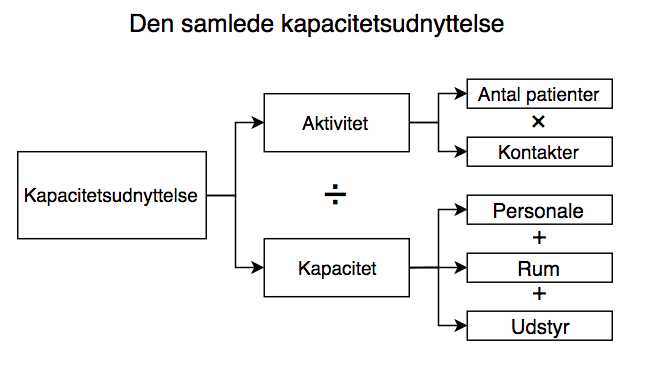
\includegraphics[scale=.45]{figures/Kapacitetsudnyttelse.png}
	\label{kapacitet}
	\flushleft
	\caption{\textit{Opdeling af den samlede kapacitetsudnyttelse. Aktivitet omfatter af antallet patienter og kontakter. Kapacitet omfatter personale, rum og udstyr. \cite{Company2013}}}
\end{figure}

\noindent
Belægning beskriver antallet af patienter, der er normeret til på en afdeling \cite{Heidmann2014}. Når en $100~\%$ belægning opnås, svarer dette til, at alle sengepladser på en afdeling er taget i brug, hvilket er fuld udnyttelse af fysisk kapacitet. Ved en belægningsgrad på over $100~\%$ betyder det, at der er flere patienter end afdelingen er normeret til, hvilket vil sige, at afdelingen yder mere end der er fysisk kapacitet til. Ved en belægningsgrad på under $100~\%$ er der omvendt færre patienter end afdelingen er normeret til, således der er tomme sengepladser og afdelingen derved ikke udnytter den fysiske kapacitet effektivt. \cite{Pauly1986} 

\section{Kapacitetsmangel}






\section{Omfang af belægning}
På ortopædkirurgisk afdeling på Aalborg Universitetshospital ses en varierende belægningsgrad fra måned til måned. Belægningsgraden er antallet af disponible senge i brug. På \figref{maxminbelaeg} ses den varierende belægning fra år $2014$ til $2015$ på ortopædkirurgisk afdeling. \cite{SDS2015}


\begin{figure}[H]
	\flushleft 
	\centering
	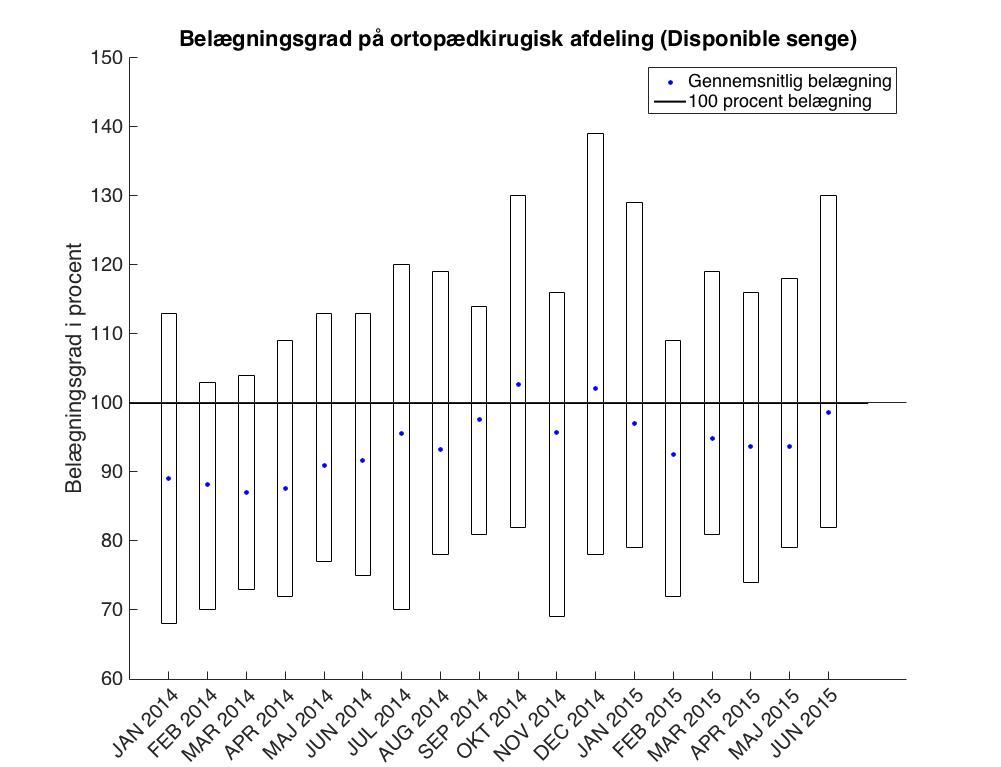
\includegraphics[scale=.45]{figures/maxminoverbelaeg.png}
	\label{maxminbelaeg}
	\flushleft
	\caption{\textit{Figuren illustrerer belægningsgraden over 18 måneder fra år $2014$ til $2015$ på ortopædkirurgisk afdeling på Aalborg Universitetshospital. Søjlerne viser belægning ift. $100\%$ belægning, dertil ses den gennemsnitlige belægning for hver måned som et punkt. \cite{SDS2015}}}
\end{figure}

\noindent
Det fremgår af \figref{maxminbelaeg}, at ortopædkirurgisk afdeling oplever en belægning hhv. over og under én ønskede belægning på $100 \%$. I december måned år $2014$ ses en maksimal belægning på $1XX \%$ og en minimums belægning på $xx \%$. Dette indikerer, at ortopædkirurgisk afdeling oplever belægning over $100 \%$ i kortvarige perioder. Da \figref{maxminbelaeg} ikke viser belægningsperioden er det uvist om, hvorvidt belægningen over $100 \%$ opleves i timer eller flere dage. Der skal herudover tages forbehold for, at \figref{maxminbelaeg} både indeholder elektive samt akutte indlagte patienter, og derfor er uvist om, hvorvidt det er akutte patienter, der resulterer i en belægningsgrad på over $100 \%$. Der ses ligeledes en gennemsnitlig belægning pr. måned på \figref{maxminbelaeg}. Denne ses hyppigst under $100 \%$ belægning, hvortil der kun ses oktober samt december i år $2014$ med en gennemsnitlig belægning på over $100 \%$ belægning. Derved opleves der ikke en gennemsnitlig belægning på over $100 \%$ i $16$ ud af de $18$ oplyste måneder. \cite{SDS2015}


For at underbygge belægningsgraden yderligere, illustrerer \figref{antaldage} antal dage pr. måned med en belægningsgrad på over $100 \%$. Denne graf er udarbejdet ud fra ortopædkirurgisk afdeling over de samme 18 måneder fra år $2014$ til $2015$ som \figref{maxminbelaeg}. \cite{SDS2015} 

\begin{figure}[H]
	\flushleft 
	\centering
	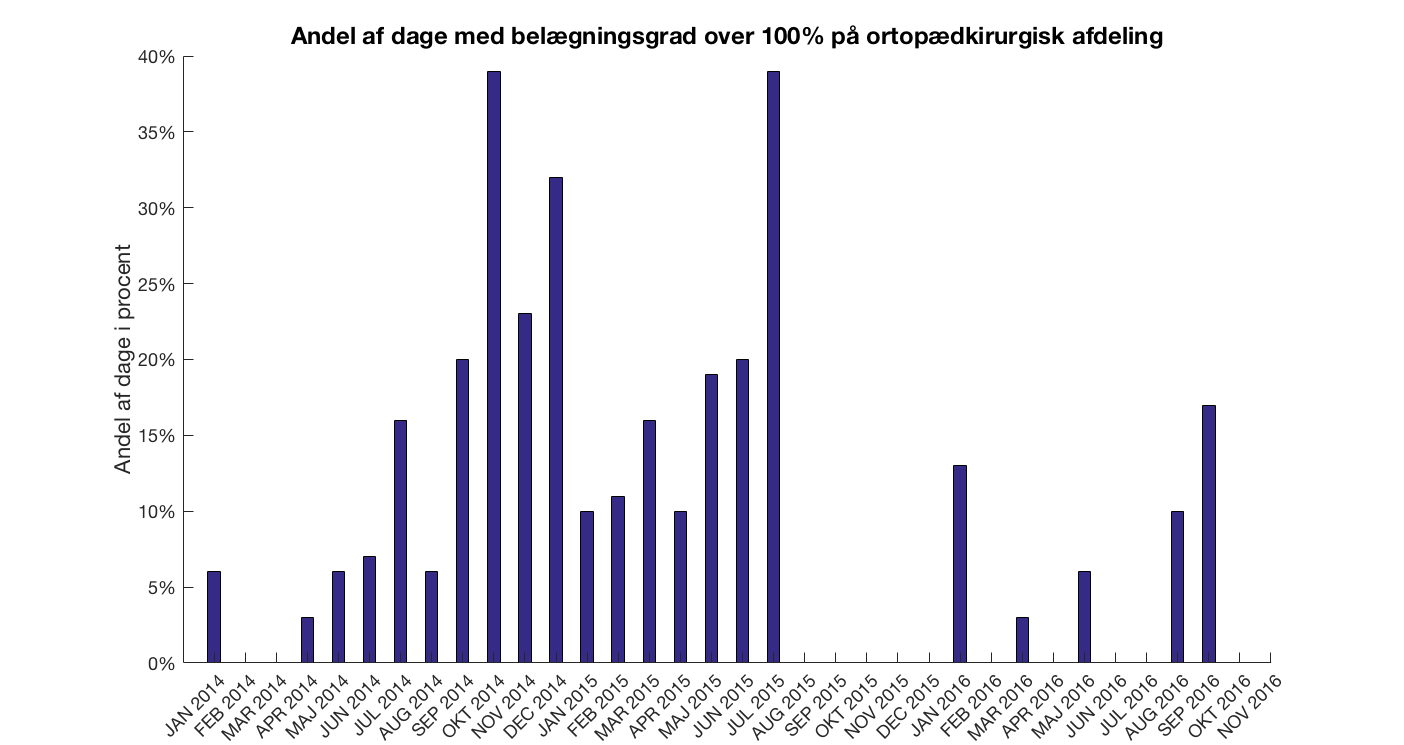
\includegraphics[scale=.7]{figures/antaldage.png}
	\label{antaldage}
	\flushleft
	\caption{\textit{Figuren illustrerer antal dage med en belægningsgrad over $100 \%$ fra januar 			$2014$ til juni $2015$ på ortopædkirugisk afdeling på Aalborg Universitetshospital. 					\cite{SDS2015}}}
\end{figure}

\noindent
Af \figref{antaldage} ses det, at der i oktober måned år 2014 opleves en belægning på over $100 \%$ i 19 dage. Det vides dog ikke, hvorvidt der er tale om én ekstra eller flere patienter, der udgør en belægningsgrad på over $100 \%$, samt hvor længe patienterne er indlagt på afdelingen. Det ses i \figref{maxminbelaeg}, at der i oktober måned år 2014 opleves en belægning på $130 \%$, hvilket kan opholdes mod de 19 dage. Det skal understreges, at begge grafer er angivet i måneder, og det er derfor uvist om, hvor mange patienter, der er indlagt pr. dag. Derudover er figurerne, \figref{maxminbelaeg} og \figref{antaldage}, udarbejdet over 18 måneder, hvilket angiveligt ikke er en repræsentativ periode for at konkludere et reelt problem på afdelingen. Dertil vides det ikke om belægningsgraden over $100 \%$ opleves som værende et problem på ortopædkirurgisk afdeling på Aalborg Universitetshospital eller om det blot er et strukturerings problem. 


% PROBLEMLØSNING
\chapter{Problemløsning}
På ortopædkirurgisk afdeling på Aalborg Universitetshospital ønskes der, på baggrund af afsnit \ref{kap}, en $100~\%$ kapacitetsudnyttelse med henblik på at udnytte de tilgængelige ressourcer optimalt. Kapacitetsudnyttelse er forholdet mellem aktivitet og kapacitet, hvoraf belægningsgraden er en betydende faktor ift. aktivitet. Det fremgår af afsnit \ref{omfang}, at belægningen på ortopædkirurgisk afdelingen er varierende, herunder opleves en ubalance i kapacitetsudnyttelse. Ved en belægning over $100~\%$ vil afdelingen opleve kapacitetsmangel, hvilket vil betyde at personalet skal yde mere end afdelingen har kapacitet til. Derimod vil afdelingen ved en belægning under $100~\%$ forårsage, at der ikke er fuld udnyttelse af personalets arbejdskraft. Da der ses ubalance i kapacitetsudnyttelsen og belægning kan dette tyde på, at der skal forekomme en effektivisering af planlægningen af patienter på ortopædkirurgisk afdeling. På baggrund af dette opstilles følgende hypotese:\\

\noindent
%\begin{itemize}
%\item 
Indlæggelsesvarigheden for patienter kan benyttes til at effektivisere kapacitetsudnyttelsen. 
%\end{itemize}

\subsection{Prædiktiv model}
For at forbedre kapacitetsudnyttelsen på ortopædkirurgisk afdelingen undersøges det, hvorvidt en prædiktiv model kan anvendes.
%Det fremgår af AFSNIT\fxnote{ref til afsnit}, at ortopædkirugisk afdeling på Aalborg Universitetshospital ikke fastholder en kapacitetsudnyttelse på $100$\%.\fxnote{snak sammen med Linette og Maria} 
Dette forventes muligt ved en forudsigelse af patienternes indlæggelsesvarighed. Aalborg Universitetshospital har i et tidligere projekt indsamlet data fra $1.000$ hospitalsindlæggelser fra ortopædkirurgisk afdeling. Disse data inkluderer bl.a. blodprøveanalyser og knoglescanninger (DXA), hvilket formodes at kunne anvendes til udvikling af en prædiktiv model. 

\noindent
Prædiktiv modellering definerer en proces, hvor en model udarbejdes med henblik på at forudsige hændelser. Denne model skal gøre det muligt at forstå og kvantificere nøjagtigheden af modellens forudsigelser ift. fremtidig data.\cite{Kuhn2013} 
Inden for sundhedssektoren er det muligt at prædiktere forskellige former for hændelser og forløb ved anvendelse af disse modeller. Dette kan eksempelvis være en forudsigelse om, hvorvidt en patient, indlagt med hjertestop, har risiko for endnu et hjertestop. Dette baseres på demografi, kost samt kliniske målinger. Et andet eksempel herpå kan være en estimering af glukosemængden i blodet hos en diabetiker, hvilket baseres på det infrarøde absorptionsspektrum af patientens blod.\cite{Hastie2008}

\noindent
Prædiktiv modellering kan opdeles i de to kategorier parametrisk og ikke-parametrisk. Forskellen på disse to kategorier ses overordnet ved om antallet af parametre kan varieres. I datasættet anvendt i projektet benyttes forskellige antal parametre for flere datapunkter og er derfor ikke-paramtetrisk.\cite{Sheskin2000}

\noindent
En prædiktiv model kan opbygges som en matematisk model eller en computerbaseret databehandlingsmodel (på engelsk: computational models). De matematiske modeller er mindre optimale at avende ved ikke-parametriske datasæt\fxnote{uddyb lidt måske}. Af denne årsag fokuserer projektet fremadrettet på computerbaseret databehandling, da denne egner sig bedst til det tilgængelige ikke-parametriske datasæt. \cite{Sheskin2000} 


\urlstyle{same}

\printbibliography
\cleardoublepage

% BILAG
%\begin{appendices}

%\end{appendices}

\end{document}
